% Generated by ASTES Journal Editorial Team
\documentclass{article} %%% use \documentstyle for old LaTeX compilers
\usepackage{geometry}
 \geometry{
 a4paper,
 total={170mm,257mm},
 left=20mm,
 top=20mm,
 }

\usepackage[english]{babel} %%% 'french', 'german', 'spanish', 'danish', etc.
\usepackage{amssymb}
\usepackage{amsmath}
\usepackage{multirow}
\usepackage{txfonts}
\usepackage{multicol}
\usepackage{booktabs}
\usepackage{mathdots}
\usepackage[classicReIm]{kpfonts}
\usepackage{graphicx} %%% use 'pdftex' instead of 'dvips' for PDF output
\usepackage{fancyhdr}
\usepackage{hyperref}
\usepackage{float}
\usepackage{microtype}
\pagestyle{fancy}
\usepackage{caption}
\captionsetup{font={footnotesize}}


%Paste this code in page 1
\fancyhead{}
\fancyhead[C]{ }
\renewcommand{\headrulewidth}{0pt }
\fancyfoot{}
\fancyfoot[L]{\href{http://www.astesj.com}{www.astesj.com}}
\fancyfoot[R]{\thepage}
%%%%%%%%%%%%%%%%%%%%%

% You can include more LaTeX packages here 

\makeatletter
\def\@xfootnote[#1]{%
  \protected@xdef\@thefnmark{#1}%
  \@footnotemark\@footnotetext}
\makeatother


\begin{document}

%\selectlanguage{english} %%% remove comment delimiter ('%') and select language if required



\begin{tabular}{p{1in}p{3.8in}p{1.2in}}  
\hspace{-1cm}
\noindent
\begin{tabular}{c}  
\includegraphics[width=2.9cm]{ASTES_Logo.jpg}\end{tabular} 	& \centering \textit{Advances in Science, Technology and Engineering Systems Journal \newline Vol. 4, No. 2, XX-YY (2019)} \\   \href{http://www.astesj.com}{www.astesj.com}  
	& \vspace{-0.6cm}  \rule{1.2in}{0.5pt} \vspace{-0.2cm} \newline \centering  \textbf{ ASTES Journal \newline ISSN: 2415-6698} \newline \rule{1.2in}{0.5pt} 
\end{tabular}


\vspace{1.8cm}






\noindent  \textbf{ \LARGE{\setlength\itemsep{0pt}A Proposal for Analog Front End Design of Contactless Smart Card-A based on Standard ISO/IEC14443-2}}

\vspace{0.2cm}

Yao-Ming Kuo\footnote[*]{Yao-Ming Kuo, Address: 25 de Mayo 1977, General San Martin, Buenos Aires, Argentina \& Email: ykuo@frba.utn.edu.ar}${}^{1,2}$, Agustín Grosso${}^{1}$, Flavio Galimberti${}^{1}$, Juan Tántera${}^{1}$, Jorge Mallo${}^{1}$ and Sebastián Verrastro${}^{1}$

\vspace{0.2cm}
 \textit{${}^{1}$Universidad Tecnológica Nacional, Electronic Engineering Department, Facultad Regional Buenos Aires, C1179AAQ, Buenos Aires, Argentina }

\vspace{0.2cm}
\textit{${}^{2}$Instituto Nacional de Tecnología Industrial (INTI), Micro and Nanoelectronics - CMNB, B1650, Gral. San Martín, Buenos Aires, Argentina}

\vspace{0.3cm}

\begin{tabular}{p{1.7in} p{0.1in} p{4.1in} }
A R T I C L E  I N F O &  & A B S T R A C T \\ 
 \cline{1-1}  \cline{3-3} \setlength\itemsep{0pt} \vspace{-0.1cm}
\textit{Article history:\newline Received: \newline Accepted:  \newline Online:  \rule{1.78in}{0.5pt} Keywords: \newline Integrated circuits \newline RFID tags \newline Smart Cards } \newline \newline  & & \vspace{-0.1cm} \textit{This paper describes a set of Analog Front End design for contactless smart cards which complies with ISO 14443-2 Type A. It has been implemented in two different technologies: Globalfoundries 130nm (GF130) and On Semiconductor 500nm (ONC5). The design and implementation of both integrated circuits (IC) were manufactured by MOSIS through the Educational Program. The Analog Front End operates at 13.56MHz with data rate 106kbps. This paper will show the simulation using Synopsys HSPICE and the corresponding test for the CMOS process GF130. }\\
 \cline{1-1}  \cline{3-3}
\end{tabular}

\vspace{0.3cm}

\begin{multicols}{2}



\section{ Introduction}

In recent years Radio Frequency Identification systems
(RFID) \cite{c1} have become very popular in many service industries,
purchasing and distribution logistics, industry, manufacturing
companies and material flow systems. In contrast
with earlier techniques like barcodes, RFID is more favored
because of its longer operation distance, higher precision,
faster processing speed and storage capabilities. With it we
can identify objects and store some data in a single silicon
chip. This paper demonstrates the RF circuits design proposal
of contactless IC card which comply with ISO/IEC14443-2 \cite{c2}
and validates the topologies with measurements. This design
satisfies the performance request with the neat circuits, and has
been implemented with 0.13um and 0.5um CMOS technology
successfully.

\section{ISO/IEC14443-2}

\subsection{Types of RF interface}

In ISO/IEC 14443-2 describes two types of RF interface about contactless IC cards which operate at 13.56 MHz: Type A and Type B. \\
In Type A, the signal from PCD (Proximity Coupling Device) to PICC (Proximity Integrated Circuit Device) is modulated in ASK (Amplitude Shift Keying) with modulation index 100\%. When receiving the data from PCD, the PICC can’t process the data because the absence of the clock source. \\
In Type B, the signal from PCD to PICC is defined to be modulated with BPSK by carrier, and the signal from PCD to PICC is modulated in ASK with modulation index 10\%, which make it possible for PICC to work continuously. Therefore, the solution given by Type B could reach higher data rate, but the design of the circuits would be more complicated. The ASK index 10\% is harder to detect than index 100\%. \\
This paper describes the circuit design for the Type A.

\subsection{Analog Front-End modules}

The contactless IC card contains two main sections \cite{c10}: RF section and Data Processing Unit (DPU). The modules in RF section are demonstrated in Fig.1, which comprises Power Supply Generator (PSG), Clock Generator (CG), Voltage Regulator (VR), Power On Reset (POR), Modulator and Demodulator.
When the PICC enters to the RF field, the signal coupled by antenna can generate power supply through PSG. The PSG consists of a rectifier and a Shunt Regulator. The VG regulates the power of PSG and gives a constant voltage to the rest of the modules. As soon as the power supply reaches the operating condition, the POR gives a low level signal to reset all the Flip-Flops of the DPU. The Modulator and Demodulator are modules that let the PCD communicate with PICC.


\begin{figure}[H]
\centering
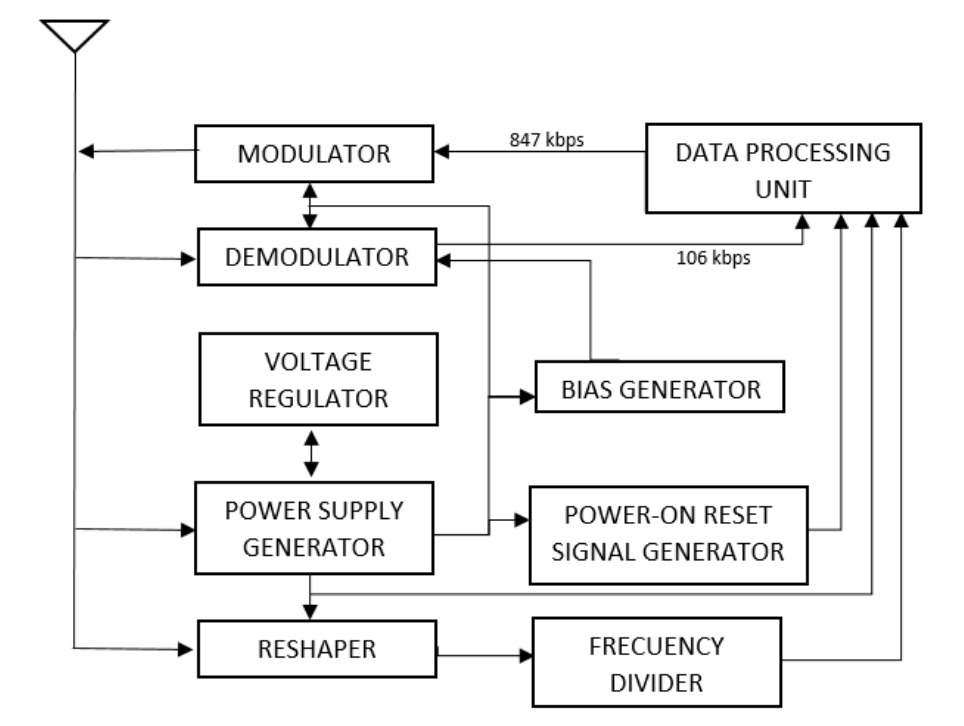
\includegraphics[scale=0.3]{Images/ImagenesTesina/modulos_rfid.png}
\caption{Analog Front-End modules}
\label{fig:modulos_rfid}
\end{figure}

\section{IC CIRCUIT DESIGN}

\subsection{Power Supply Generator (PSG)}

The PSG is divided into two parts: alternating source rectification (13.56 MHz) and power limitation. The first part rectifies the magnetic field induced from the reader. A rectifier is implemented with NMOS transistors functioning as a diode. Figure \ref{fig:rectifier} shows the implemented topology.

\begin{figure}[H]
\centering
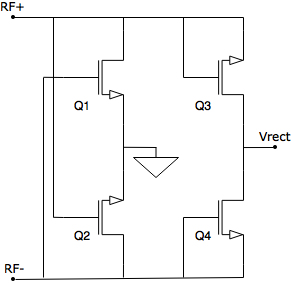
\includegraphics[scale=0.6]{Images/ImagenesTesina/circuitos/Rectifier.png}
\caption{Full-wave rectifier with NMOS transistors}
\label{fig:rectifier}
\end{figure}

It should be noted that the voltage drop on the rectifier inversely depends on the MOS channel width (W). The wider W is the less voltage falls at this stage. Logically, the limitation in this case is the area. The second part protects the chip, since in order to be ISO / IEC 14443-2 standard-compliant, the PICC must be able to work under different magnetic field strengths (1.5-7.5 A/m rms). Figure  \ref{fig:shunt} shows the topology.

\begin{figure}[H]
\centering
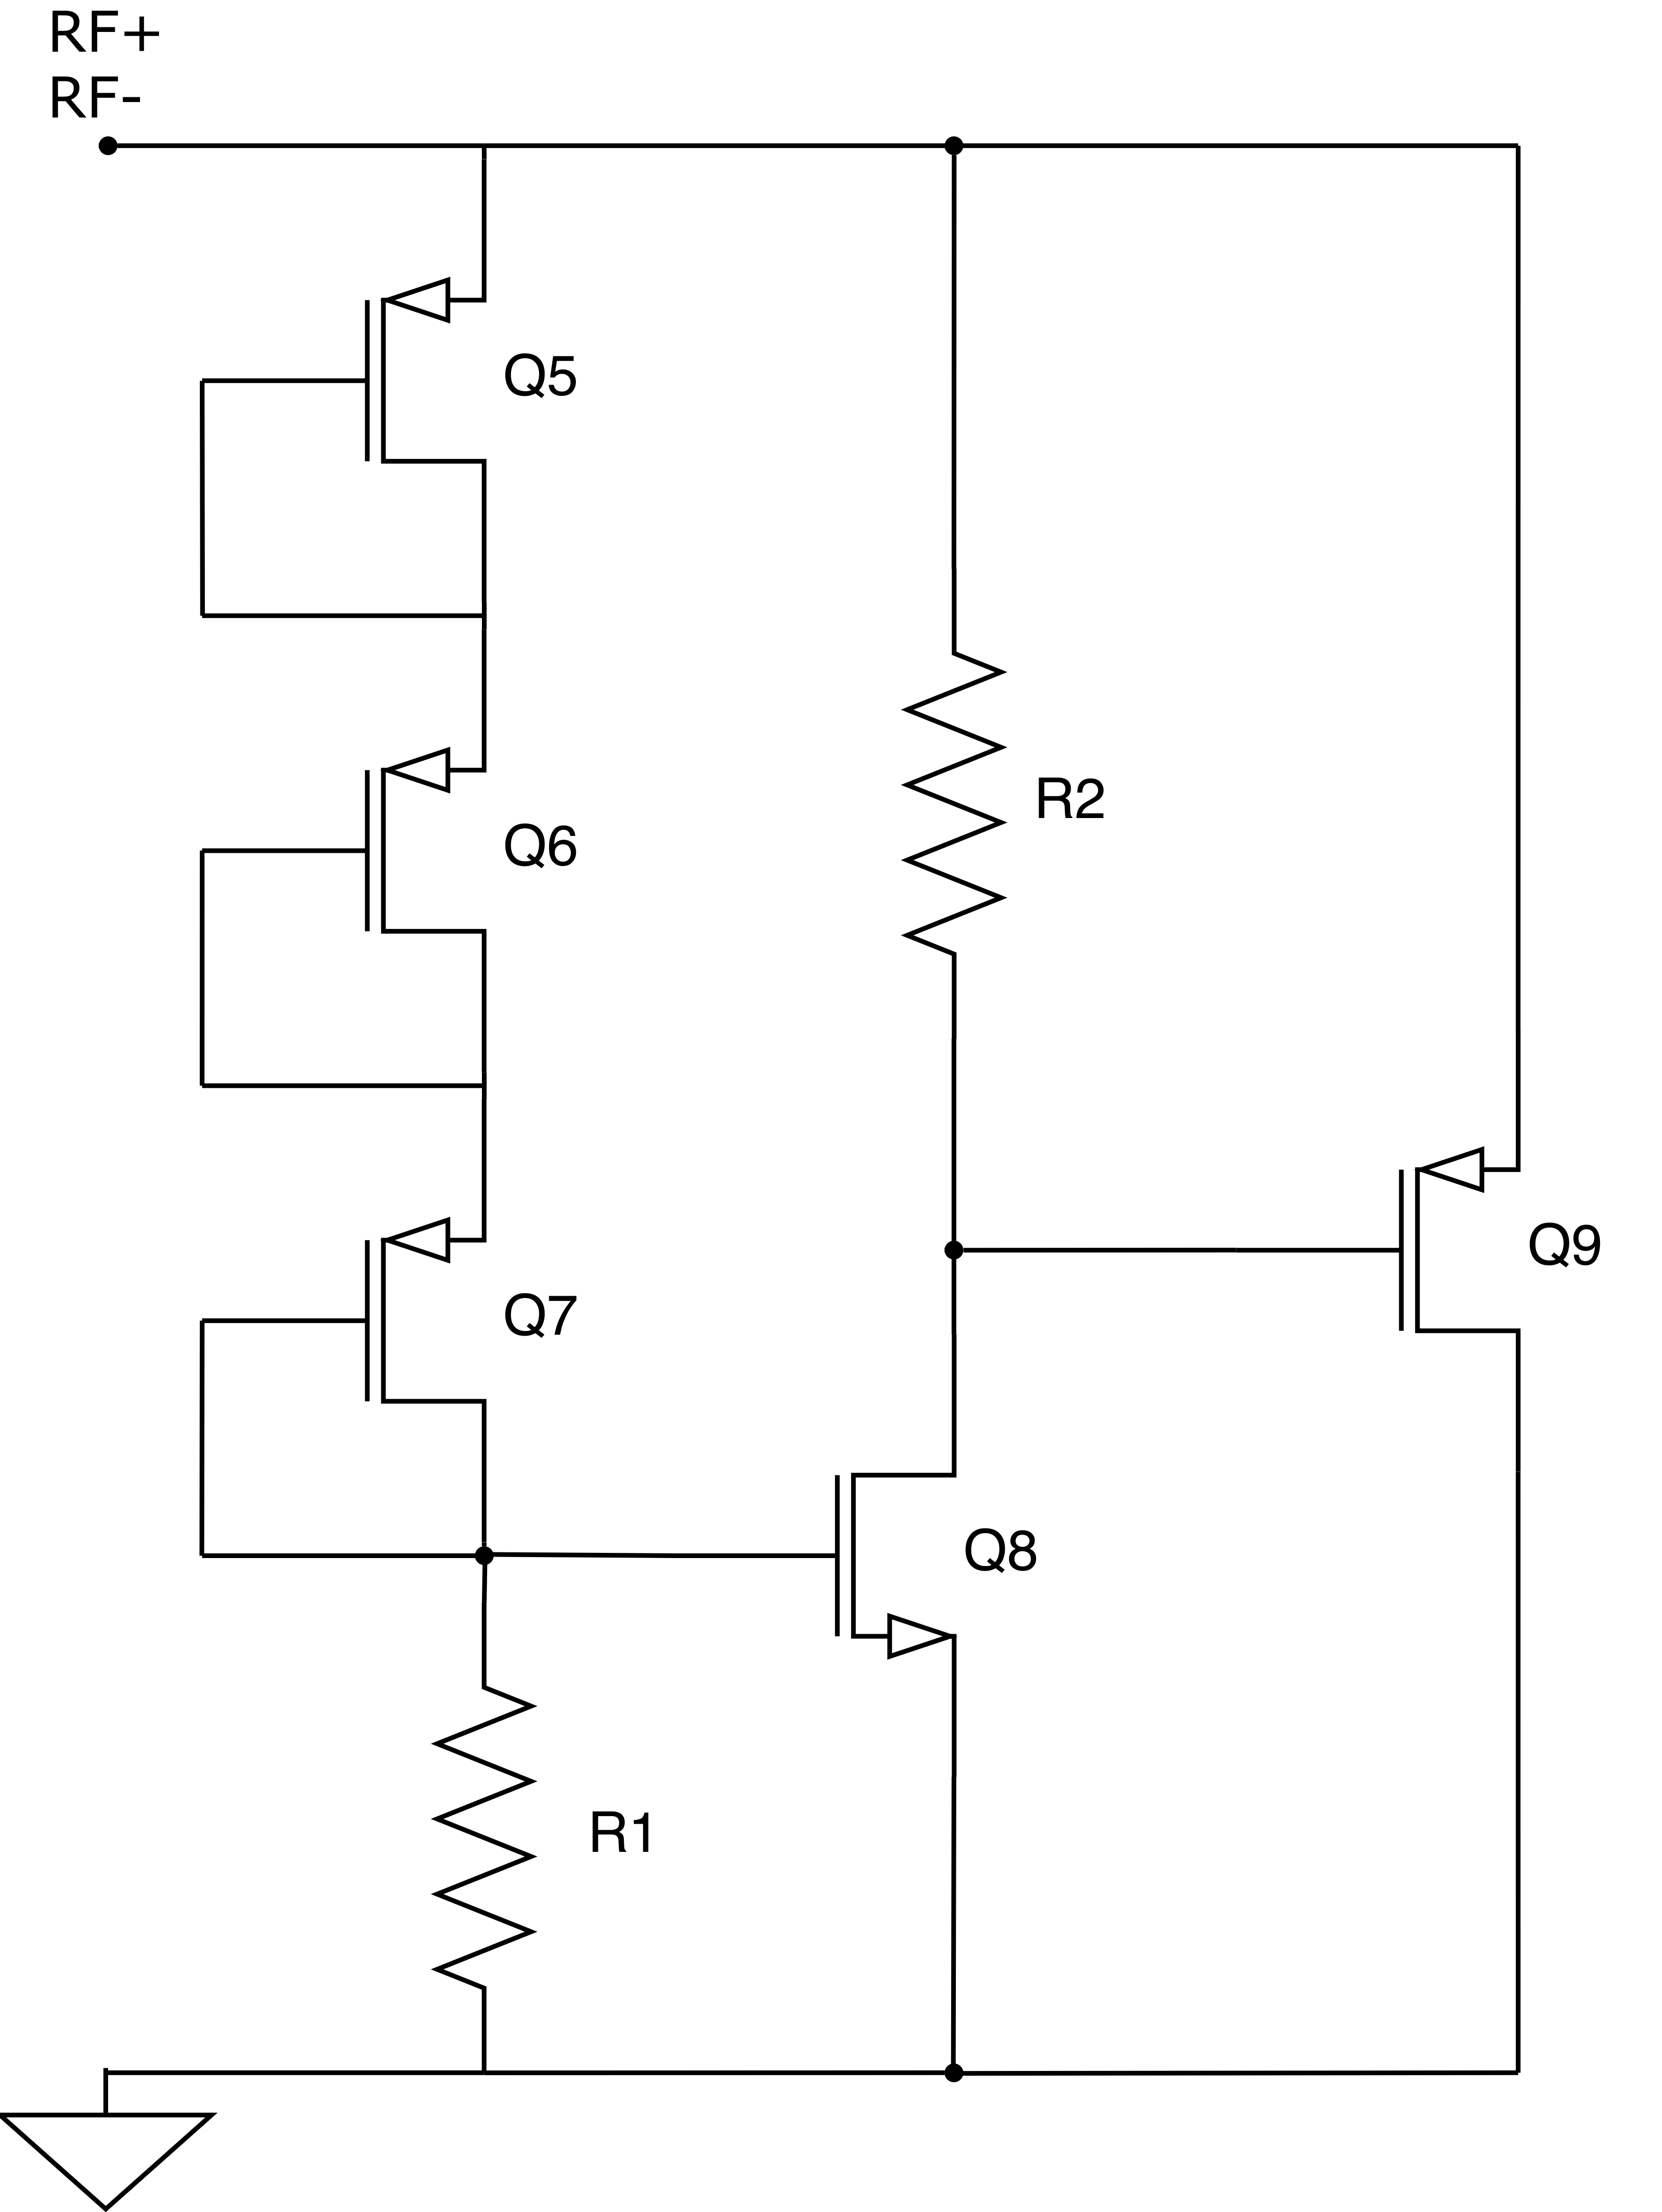
\includegraphics[scale=0.045]{Images/ImagenesTesina/circuitos/Shunt.png}
\caption{Power limiter - Shunt}
\label{fig:shunt}
\end{figure}

When a voltage that is higher than the threshold voltage appears across the terminals of the module, the shunt limiter turns Q9 transistor on, what means that this transistor works ideally only in cut-off and saturation modes. 
Considering that both used technologies have different operating voltages (3.3 to 5V for ONC5 and 1.2 to 2.5V for GF130), the threshold voltages vary. Figures \ref{fig:shunt_500} and \ref{fig:shunt_130} show the threshold voltages for each technology.

For ONC5 technology the circuit turns on at 4.5 V and for GF130 at 2.8 V. A 400 pF capacitor is located between the rectifier and the shunt. This capacitor depends on each technology operating voltage and process.
\begin{figure}[H]
\centering
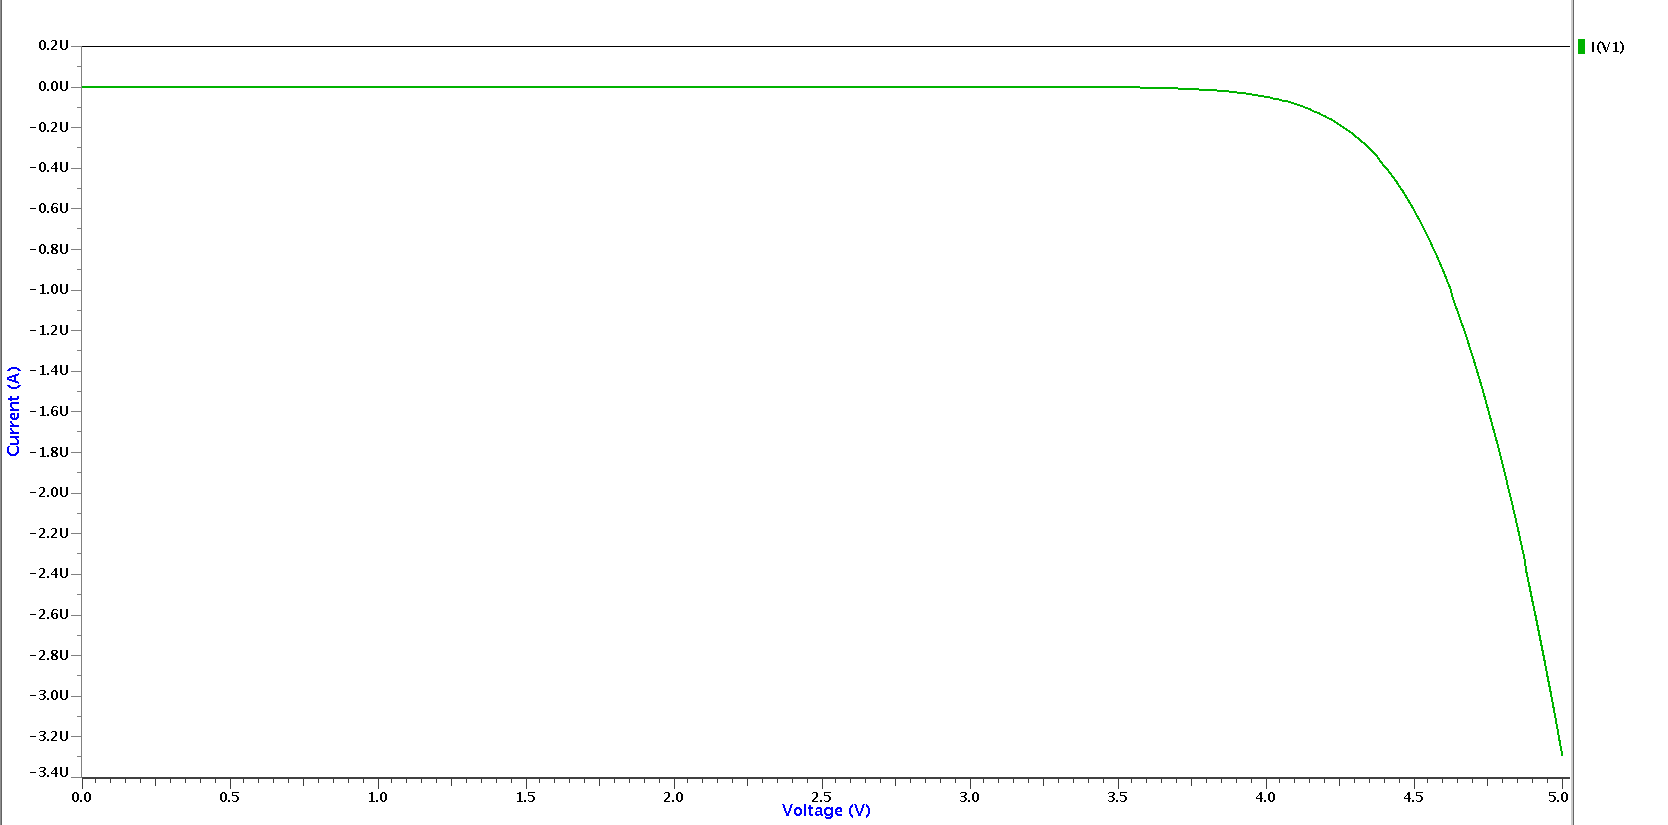
\includegraphics[width=0.9\linewidth]{Images/ImagenesTesina/simulaciones/shunt_500.png}
\caption{Threshold voltage (ONC5)}
\label{fig:shunt_500}
\end{figure}

\begin{figure}[H]
\centering
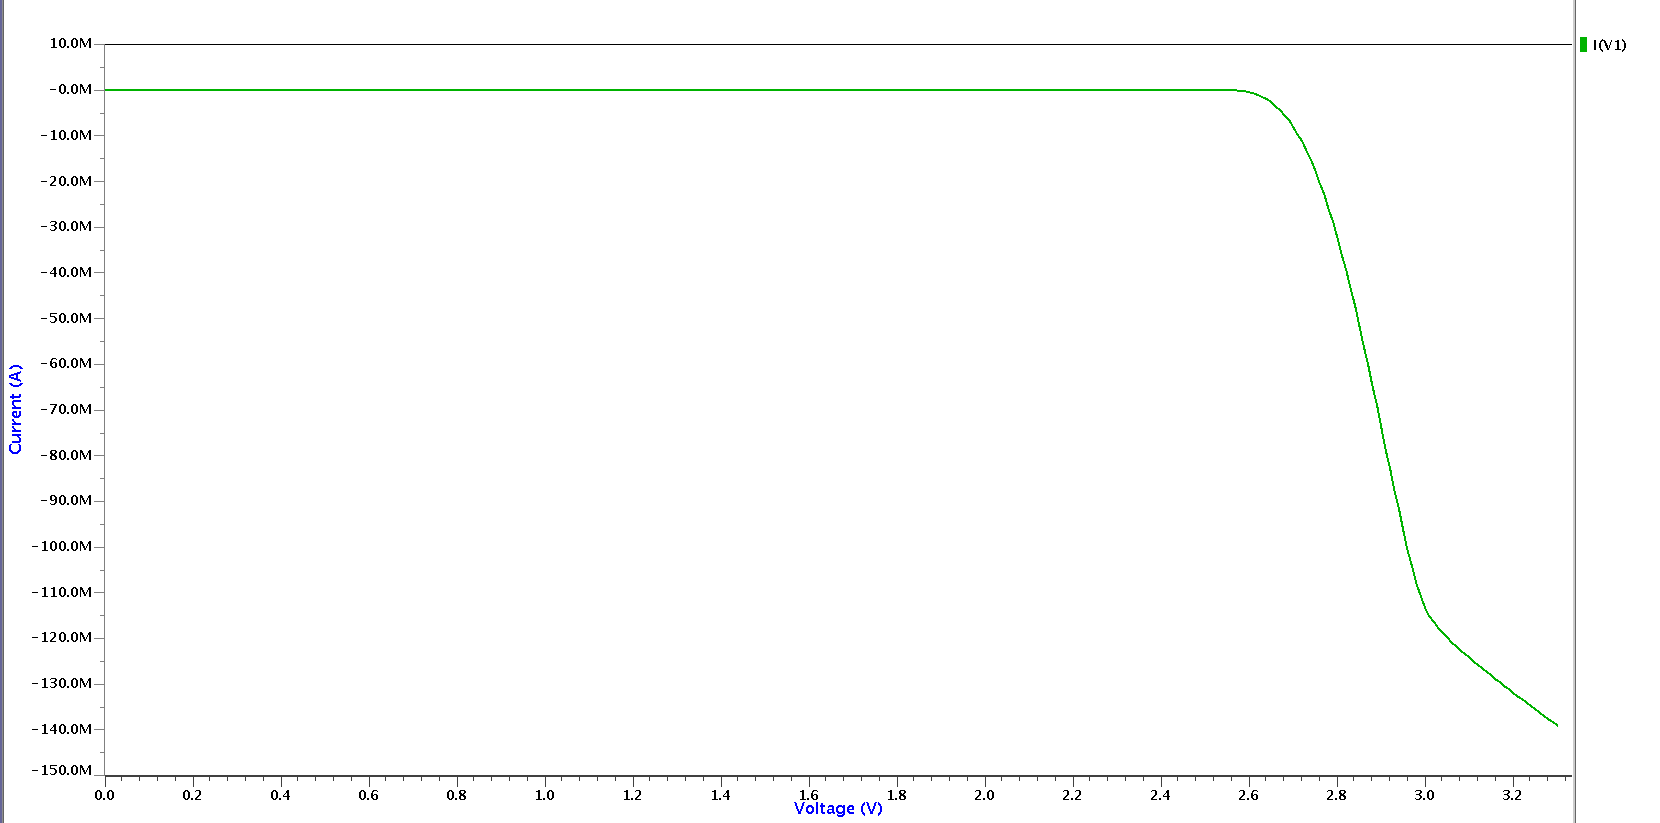
\includegraphics[width=0.9\linewidth]{Images/ImagenesTesina/simulaciones/shunt_130.png}
\caption{Threshold voltage (GF130)}
\label{fig:shunt_130}
\end{figure}

\subsection{Clock Generator (CG)}
The clock generator obtains the clock from the antenna, since the reader emits a frequency of 13.56 MHz $\pm$7kHz, as specified in ISO/IEC 14443-2 standard. The module (figure  \ref{fig:clock_gen}) consists mainly of two D type Flip-Flop (that act as a clock divider by 2) and an XOR gate.
It works basically taking advantage of the phase difference between the voltages across the terminals of the antenna with respect to ground (180 degrees of phase difference). Then it is sent through the D flip-flop and the XOR to recover the clock (figure 
\ref{fig:clock_gen_sim}).
\begin{figure}[H]
\centering
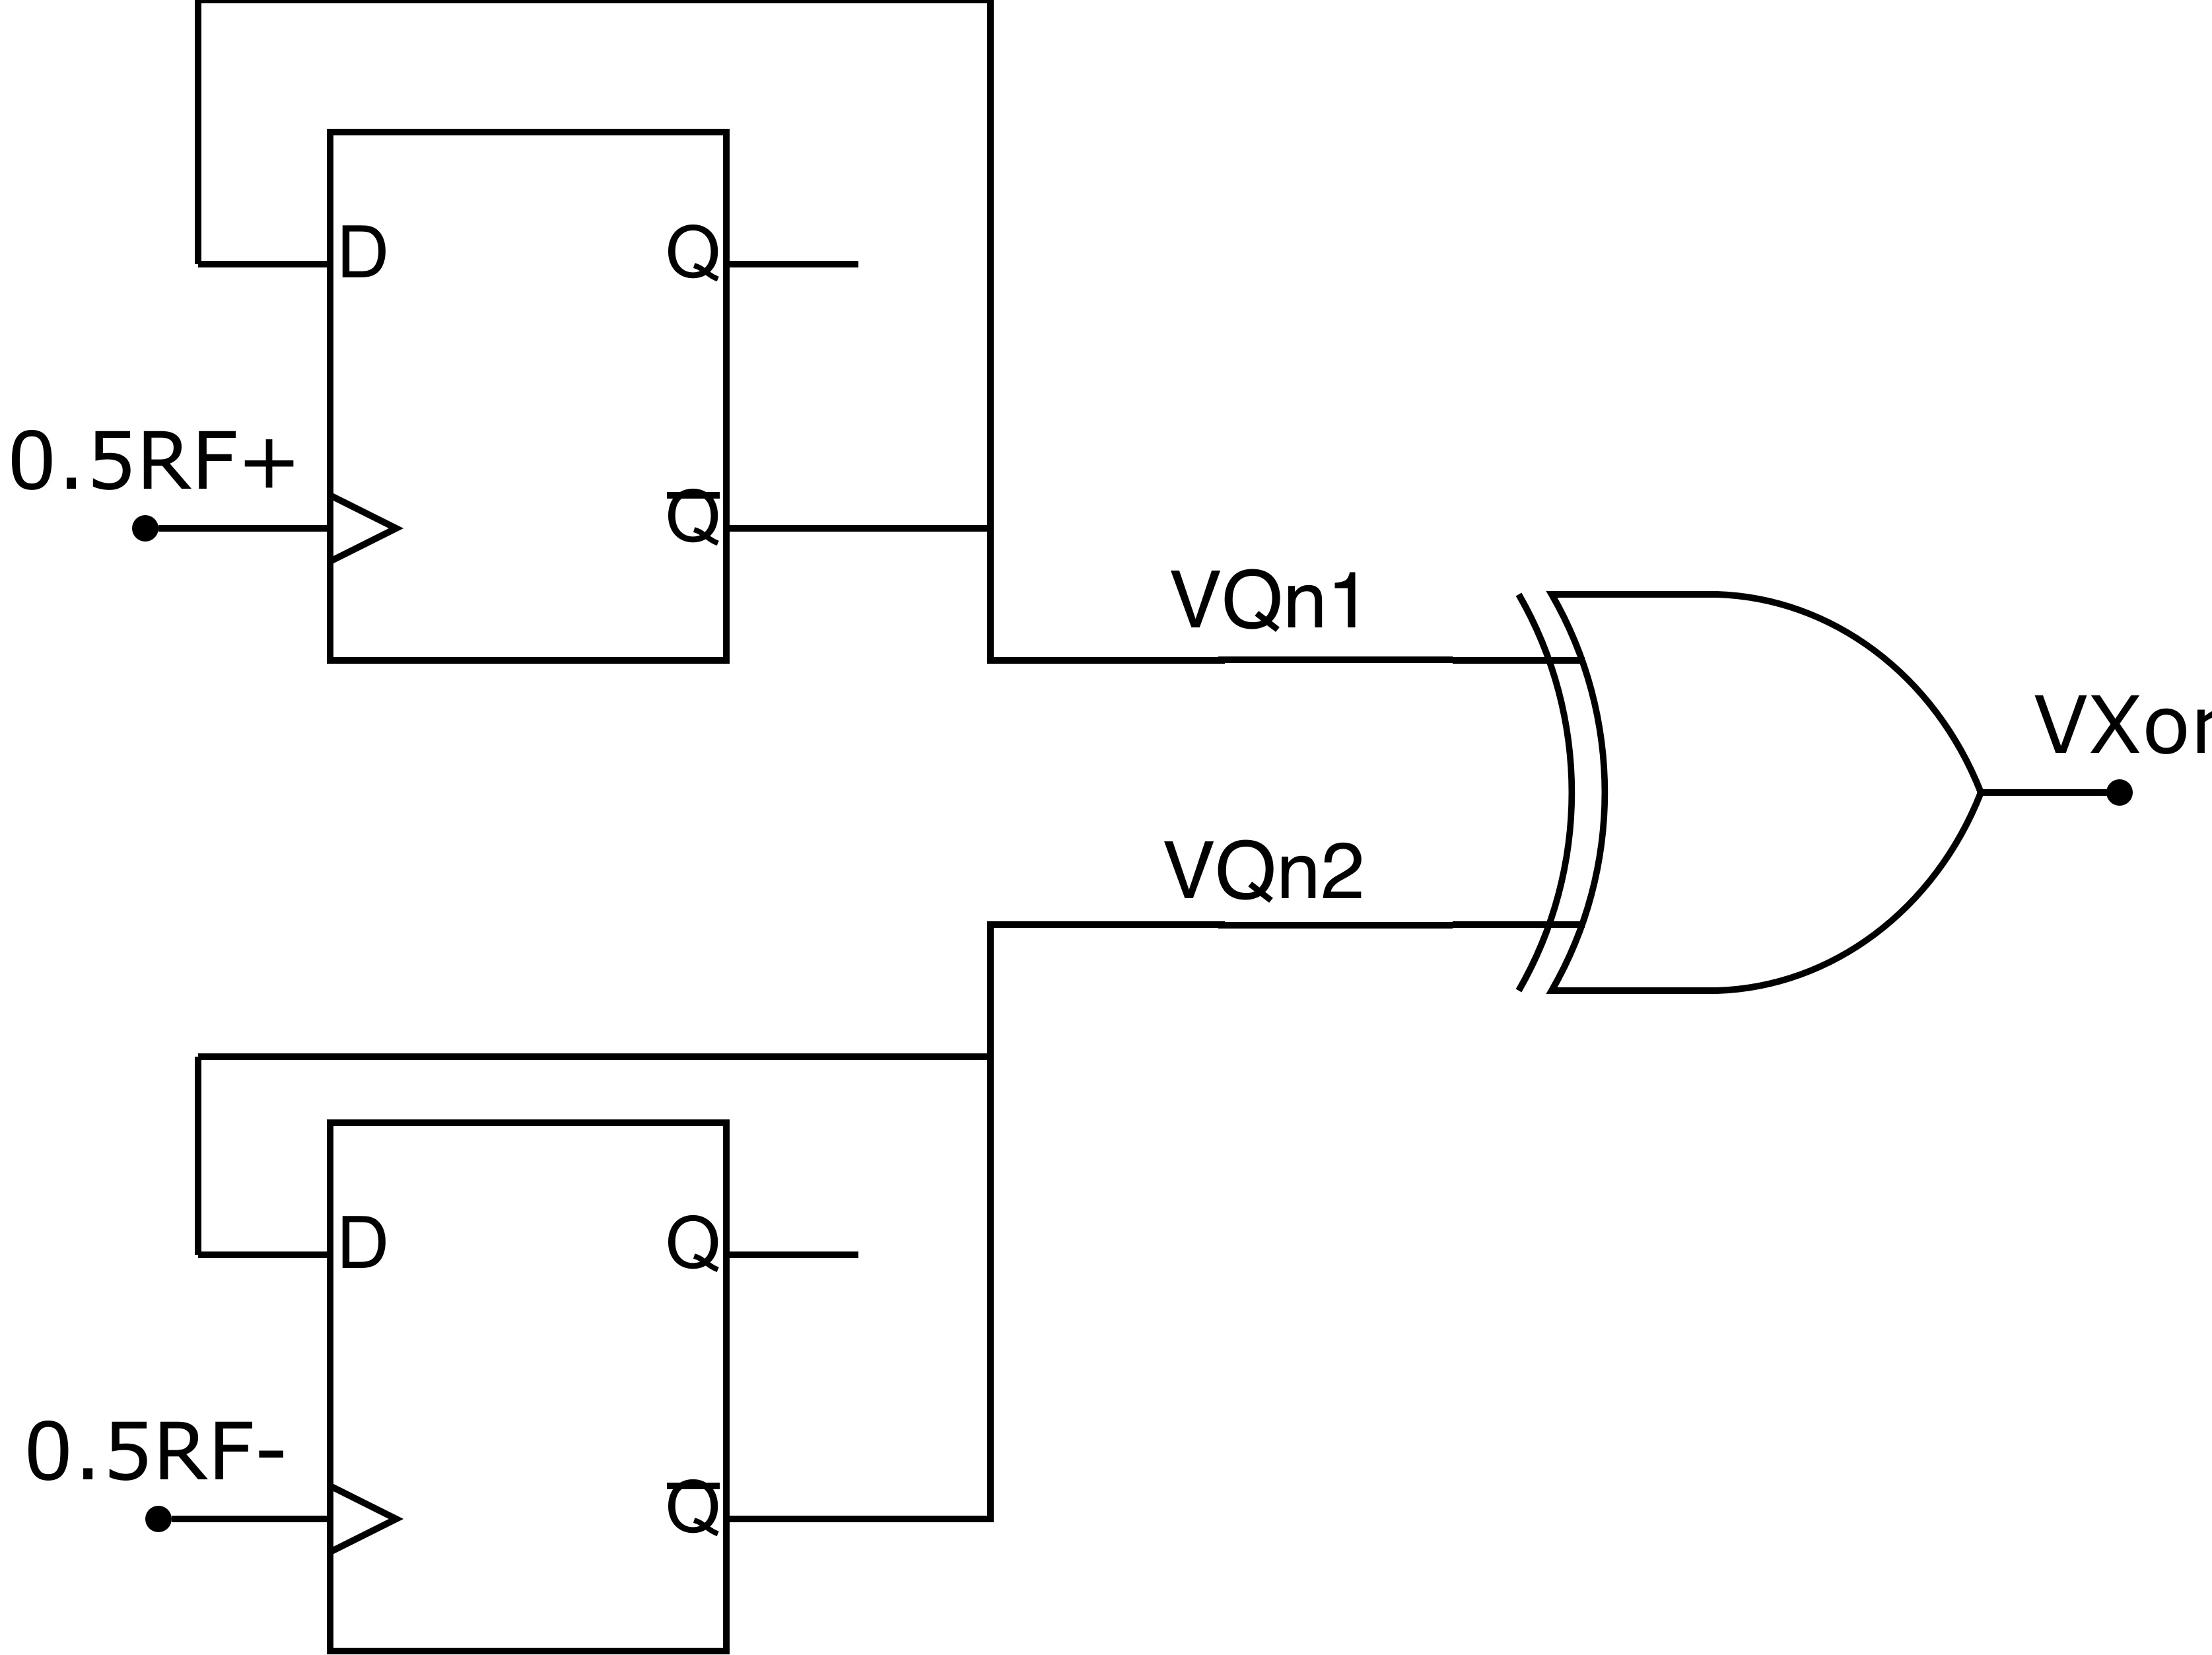
\includegraphics[width=0.5\linewidth]{Images/ImagenesTesina/circuitos/CLK.png}
\caption{Clock generator}
\label{fig:clock_gen}
\end{figure}

\begin{figure}[H]
\centering
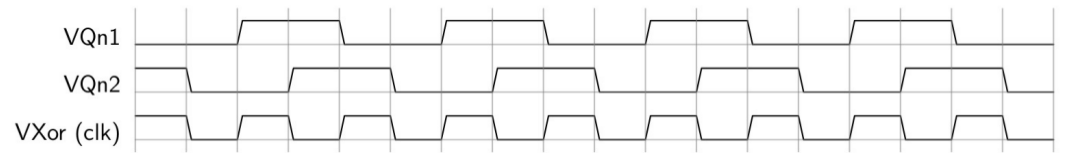
\includegraphics[width=0.9\linewidth]{Images/ImagenesTesina/circuitos/clk_sim.png}
\caption{Clock generator (Simulation)}
\label{fig:clock_gen_sim}
\end{figure}

\subsection{Voltage Regulator (VR)}
The VR regulates the voltage coming from the PSG and provides a constant, continuous voltage at the module output. This module powers the rest of the modules of the chip. The topology of the VR can be seen in figure \ref{fig:ldo}. This module consists mainly of three parts: an operational amplifier (OP-AMP) that is used as an error amplifier (works as regulation, amplifies the difference between a known reference voltage with respect to the output voltage), an output serial transistor used as a current amplifier and R3-R4 which are used as a resistive voltage divider (equation \ref{eq:vref}).  

\begin{figure}[H]
\centering
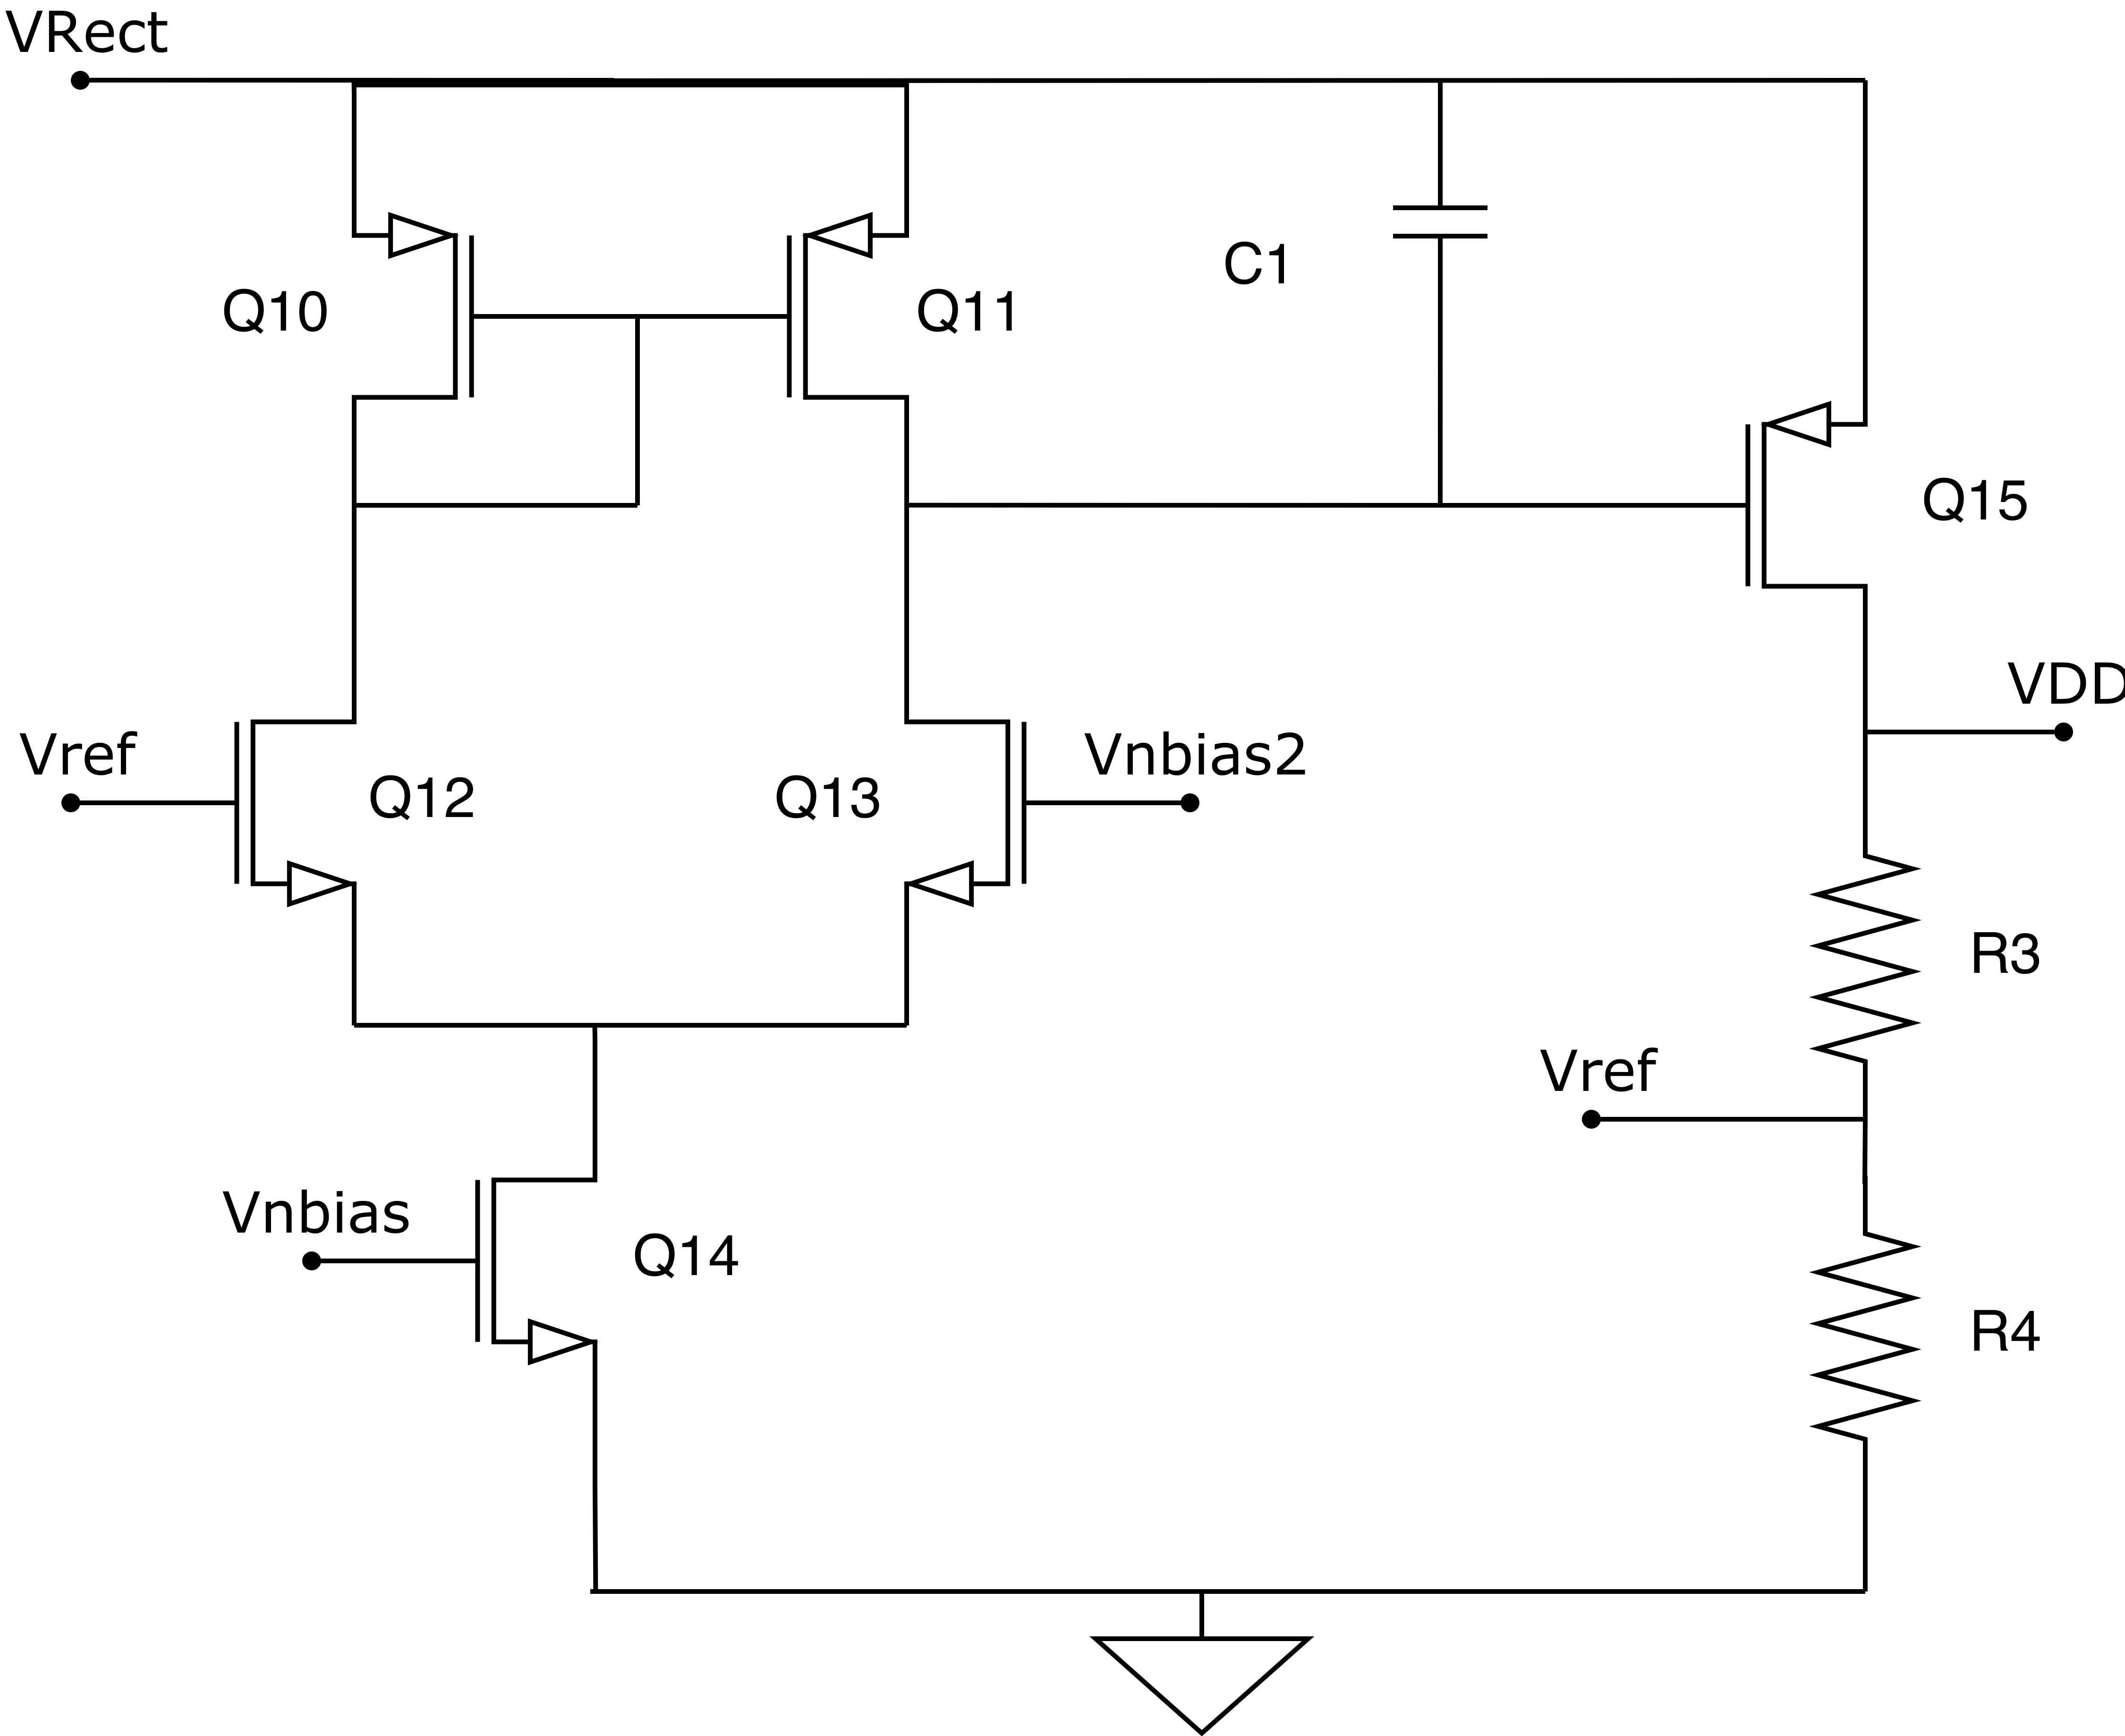
\includegraphics[width=0.8\linewidth]{Images/ImagenesTesina/circuitos/LDO.png}
\caption{Voltage regulator}
\label{fig:ldo}
\end{figure}

\begin{equation} \label{eq:vref}
VDD = Vref*(1+R3/R4)
\end{equation}

\subsection{Modulator}
The Modulator carries the signal from the PICC to the PCD module. There are two different types of load modulation: resistive and capacitive modulation. Both types create a subcarrier next to 13.56MHz. The NMOS transistors are switched on and off in time with the encoded data. This varies the load (resistive) or resonance frequency (capacitive) of the transponder. 
If variations are generated at a high frequency, two spectral lines are created at a distance of $\pm \textit{fs}$ around the transmission frequency of the PCD. The voltage variations observed in the PCD are typical of the amplitude shift modulation that is generated through the variations of the load in the PICC. The ASK (Amplitude-shift keying) is developed through the variation of the carrier signal between two amplitude values, that is, between two states, at a frequency of $\pm \textit{fs}$. ASK modulation has similar features to the well-known AM modulation (amplitude modulation). Like AM, ASK is linear, easy to implement and the data sent reconstruction is relatively simple.


\begin{figure}[H]
\centering
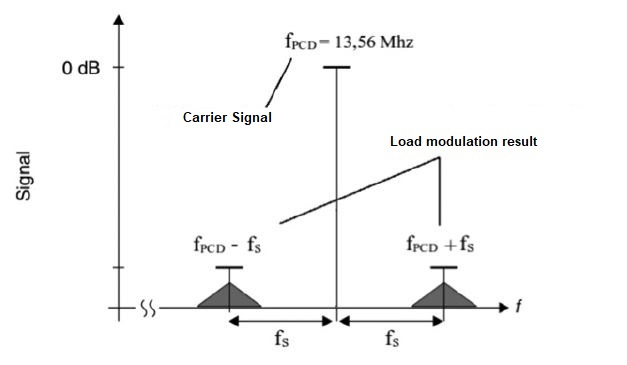
\includegraphics[scale=0.5]{Images/ImagenesTesina/Antecedentes/Modulacion_Carga_2.JPG}
\caption{Frecuency spectrum of load modulation }
\label{fig:Mod_carg}
\end{figure}

\subsubsection{Capacitive Modulator}

This module adds capacitors in parallel to the resonant circuit of the PICC in one of the $V_Data$ states, while, during the other logical level, the resonant circuit is not affected. This capacity variation causes a minimal mismatch between devices that affects the energy transfer between them and then appears as a voltage variation in the PCD antenna.
\begin{figure}[H]
\centering
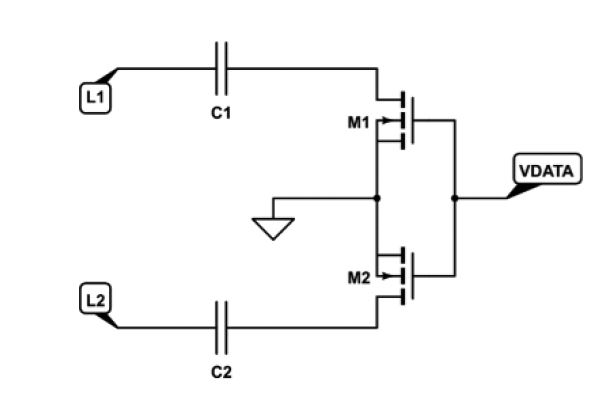
\includegraphics[scale=0.5]{Images/ImagenesTesina/Antecedentes/Modulacion_Carga_Cap.JPG}
\caption{Capacitive Load Modulator.}
\label{fig:Mod_carg_cap}
\end{figure}

\subsubsection{Transistors-only Resistive Modulator}
Looking for a higher modulation index (in this aspect the Modulator capacitive is weak) an resistive modulation topology was analyzed, in which the NMOS output resistance is used (Figure  \ref{fig:Mod_carg_trans}). As it has a low impedance, when it is connected in parallel to the resonant circuit and the load of the other modules connected to this circuit, the overall impedance decreases significantly. If the NMOS output impedance is varied at a frequency of $f_s$, a load modulation is obtained. During the analysis focused on the transistors and their behavior during modulation, current peaks were detected (Figure \ref{fig:Picos_Cor}) in the drain of each of the transistors, which could affect these devices after a considerable use. These peaks are generated because, in the simulations, $V_{Data}$ signal rise and fall times are very small values. In spite of the fact that in practice these values tend to be higher, what would decrease the peaks, we tried to add a safety margin to the circuit.

\begin{figure}[H]
\centering
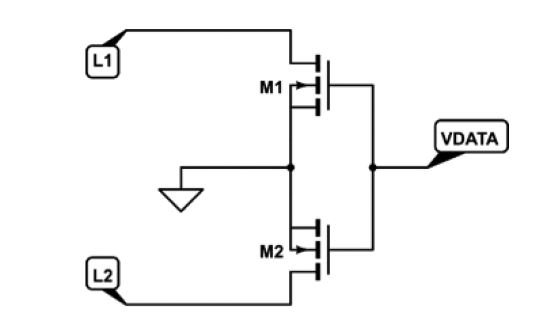
\includegraphics[scale=0.5]{Images/ImagenesTesina/Antecedentes/Modulacion_Carga_Trans.JPG}
\caption{Resistive Load Modulator.}
\label{fig:Mod_carg_trans}
\end{figure}

\begin{figure}[H]
\centering
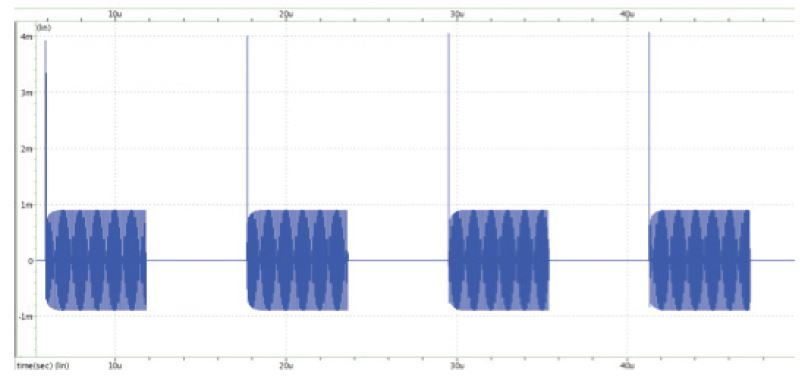
\includegraphics[scale=0.4]{Images/ImagenesTesina/Antecedentes/Picos_Corriente.JPG}
\caption{Current in the NMOS M2 drain in the topology of the Figure  \ref{fig:Mod_carg_trans}.}
\label{fig:Picos_Cor}
\end{figure}


\subsubsection{Resistive Modulator with Resistors}
In order to protect the transistors against unexpected currents peaks, the topology shown in Figure  \ref{fig:Mod_carg_trans} was modified using two resistors that not only protect the NMOS drains but also does not decrease significantly the modulation obtained with the previous topology. The final circuit (which was manufactured) was finished as it is shown in Figure \ref{fig:Mod_carg_res}. To increase the functionality range, the circuit was subjected to Monte Carlo method simulations and also through corners (extremes of the process) that contain possible variations in the characteristics of the transistors caused by the IC manufacturing process.
\begin{figure}[H]
\centering
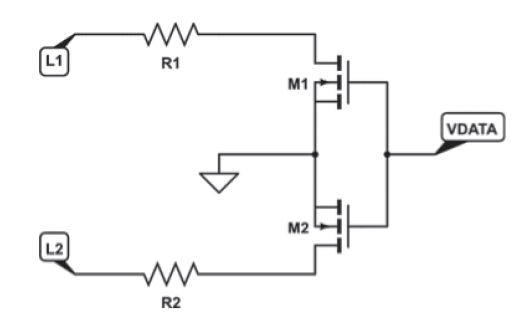
\includegraphics[scale=0.5]{Images/ImagenesTesina/Antecedentes/Modulacion_Carga_Res.JPG}
\caption{Resistive Modulator with Resistors.}
\label{fig:Mod_carg_res}
\end{figure}

\subsection{Demodulator}

The Demodulator recovers the digital frame transmitted from the PCD module. An Envelope Extractor (EE) circuit \cite{c4} is needed to extract the data. The digital signal is recovered by connecting the output of the EE with the input of the buffer. The circuit is shown in Fig. \ref{fig:demod}. A Demodulator is made up of a signal rectification and envelope detection block . Then, if necessary, a signal filtering stage to avoid errors in the next phase of signal processing due to high frequency variations on the envelope signal and, in the end of the demodulation process, the filtered signal is sent to a Schmitt Trigger  \cite{c6} finally obtaining the signal representing the data sent by the PCD. 
Apart from the Schmitt Trigger and a low pass filter, the topology under analysis (fig  \ref{fig:Demod2}) has a comparator and an enabling input. It also has the advantage of being able to adjust the level of the comparator externally. The disadvantage is that the operational amplifier designed has a response time (Slew Rate) much larger than the Schmitt Trigger.

\begin{figure}[H]
\centering
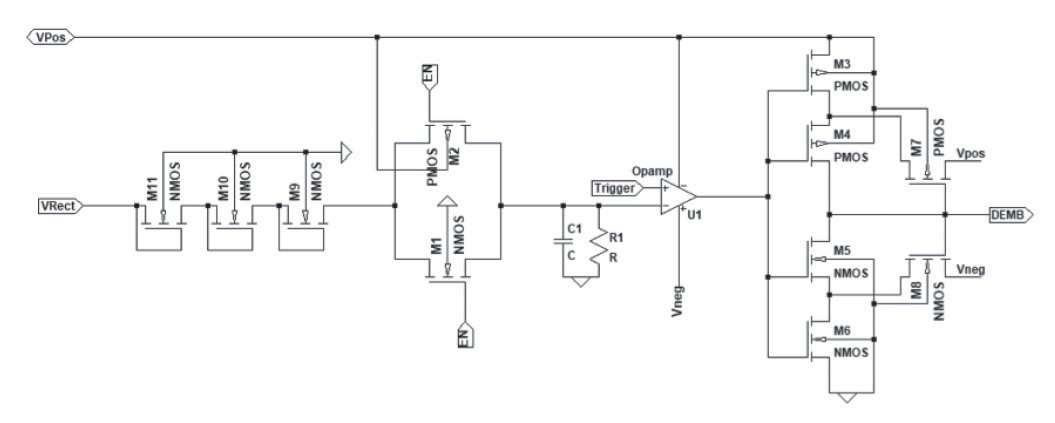
\includegraphics[scale=0.3]{Images/ImagenesTesina/Antecedentes/Demod2.PNG}
\caption{Schematic circuit of the Demodulator topology used.}
\label{fig:Demod2}
\end{figure}

\subsubsection{Rectifier and envelope detector}
In this stage, a topology of an AM Modulator (Modulated Amplitude) was used. This is a circuit known for its simplicity, consisting of a rectifier and a detector (Resistor and Capacitor in parallel). See Fig. \ref{fig:Detect} .
\begin{figure}[H]
\centering
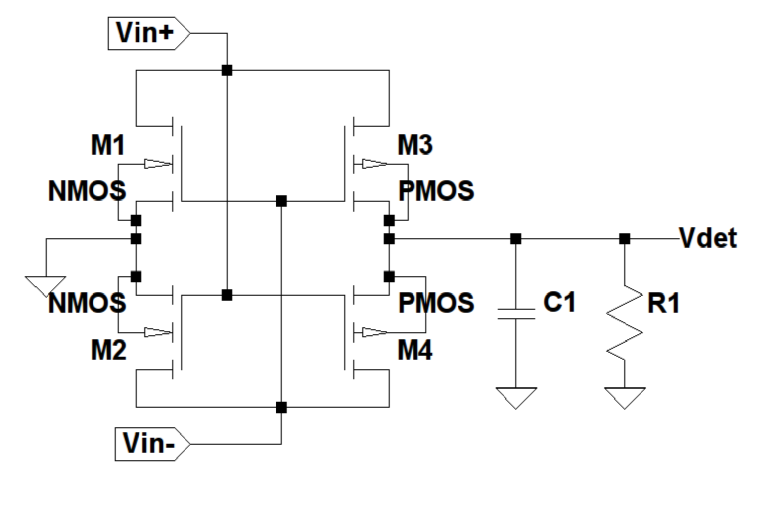
\includegraphics[scale=0.2]{Images/ImagenesTesina/Antecedentes/Detect_RC.png}
\caption{Rectifier and envelope detector.}
\label{fig:Detect}
\end{figure}
For a simpler analysis, a diode was used as a rectifier. Taking into account that the envelope detector consists of a resistor and a capacitor, it presents a time constant  $\tau = RC$. Considering a carrier signal with a frequency equal to  $f_c = 13.56 MHz$, the capacitor is discharged between each carrier peak, following the following equation:

\begin{equation} \label{eq:vref}
V'_{peak} = V_{peak}e^{-\frac{t}{\tau}}
\end{equation}

Where $T = \frac{1}{fc}$. Assuming $T << \tau$, then:

\begin{equation} \label{eq:vref}
{\bigtriangledown V} \simeq V{peak}\frac{T}{\tau} = \frac{V_{peak}}{f_c \tau}
\end{equation}


When the signal is modulated in ASK, its voltage goes from a defined voltage value to a much lower value (zero Volt in this case). The voltage drop in the envelope detector, from one value to another, can be seen in the following equation:

\begin{equation} \label{eq:vref}
V_{drop} = V_{peak}e^{-\frac{t}{\tau}}
\end{equation}


The detector circuit can be analyzed in response to the mentioned voltage change  using the previous equation. Depending on the RC’s time constant, the circuit can be more or less sensitive to the change in voltage. In practice, a good relationship between the detector’s response facing a voltage change at the modulating frequency and the ripple at the carrier frequency, a time constant is adopted which must be inside the following interval:

\begin{equation} \label{eq:tauRC}
   \frac{1}{f_c} << \tau << \frac{1}{f_m}
\end{equation}

Then, having 13.56 MHz as $f_c$ (carrier frequency) and 106 kHz as $f_m$ (modulating frequency) the following component values were chosen:
$$R = 5 k\Omega ; C = 30 pF$$
As a result, the relationship between frequencies and $\tau$ is:
$$\frac{1}{13.56MHz}<<1.5.10^{-7}s<<\frac{1}{106kHz}$$

\begin{figure}[H]
\centering
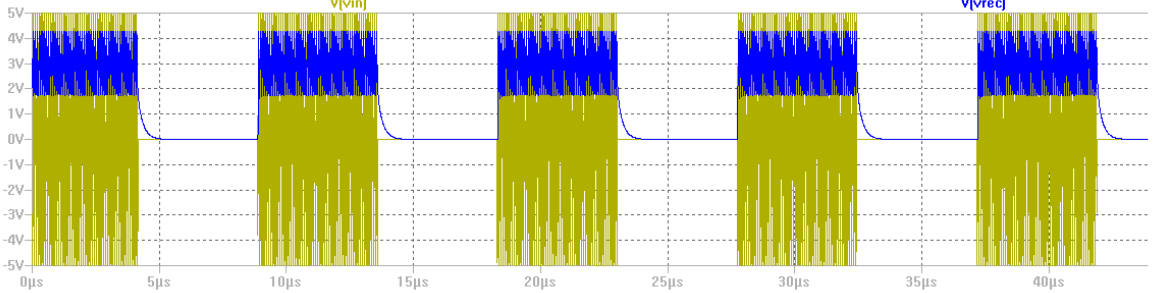
\includegraphics[scale=0.2]{Images/ImagenesTesina/Antecedentes/Sim_Detect.png}
\caption{Input signal and output signal from the envelope detector $\tau = 0,15\mu$ S.}
\label{fig:Sim_detect}
\end{figure}
 
\subsubsection{Low Pass Filter}
To prevent errors to occur in the next stage due to not desired voltage variations, the output signal of the detector is passed through an RC filter (simple low pass filter) which purpose is to reduce the ripple at 13.56 MHz. The cutoff frequency of the filter must be below the carrier frequency, so as to filter it and above the modulating frequency, so as not to affect the envelope. So:
$$106kHz<<f_c<<13.56MHz$$
$$f_c = \frac{1}{2\pi RC} \approx 3.2MHz$$
$$R = 10 k\Omega ; C = 6 pF$$

\begin{figure}[H]
\centering
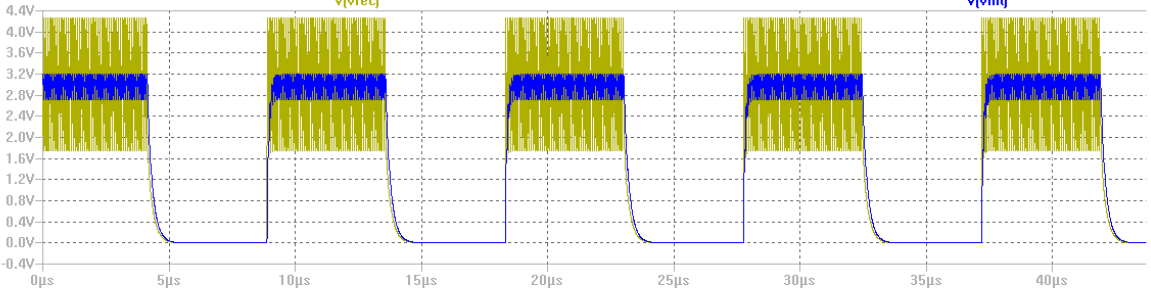
\includegraphics[scale=0.2]{Images/ImagenesTesina/Antecedentes/Sim_RC.png}
\caption{Ripple filtering at 13.56MHz with an RC filter.}
\label{fig:Sim_RC}
\end{figure}

\subsubsection{Schmitt Trigger}
Since the output signal of the Demodulator will then enter a digital system, it must be free of noise and distortion in order to avoid errors in the information and, therefore, in the whole system information management. A way to digitize a signal, removing the disturbances that it brings, is through of a Schmitt Trigger. This type of trigger is characterized by its bistable nature and by the use of a hysteresis that governs state changes. The topology chosen is a double CMOS transistor inverter with the addition of a pair of transistors that define state change points in hysteresis. This topology has the advantage of being able to choose the trigger points of the system by choosing the aspect ratio of the transistors involved. The width and length of the transistors channel’s ratio, has an effect on the hysteresis of the trigger.

\begin{figure}[H]
\centering
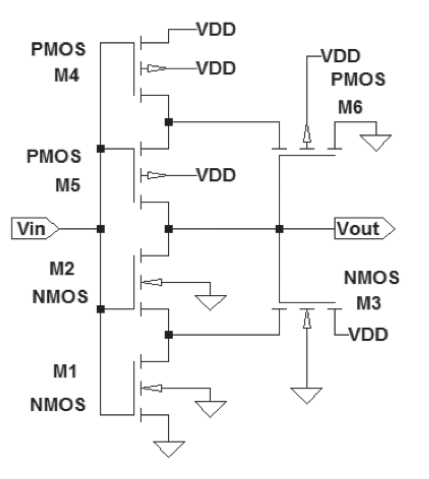
\includegraphics[scale=0.4]{Images/ImagenesTesina/Antecedentes/Schmitt_Trigger.PNG}
\caption{CMOS Schmitt Trigger.}
\label{fig:Schmit}
\end{figure}

When the circuit’s input (Fig. \ref{fig:Schmit}) is 0V, the $M_4$ and $M_5$ transistors will be driving, while $M_1$ and $M_2$ will be cutoff. Under that condition, the output will be high ($V_{out} = V_{DD}$). When the input voltage starts to rise and reaches the threshold voltage of transistor $M_1$, it will start to drive, but $M_2$ will remain cutoff. $M_1$ will tend to lower the node between itself and $M_2$ to GND, while $M_3$, which has $V_{DD}$ in its gate, will tend the node to $V_{DD}$ . Then, when the input signal exceeds $M_2$ threshold voltage, it will start to drive and the output will have 0V, referring the input voltage that triggers the output to low level such as $V_{IH}$ (limit voltage that is admitted as a logical one). Something similar happens with the upper branch of the inverter when the input voltage starts to decrease. Transistors $M_4$ and $M_6$ will tend the node to $V_{DD}$  and GND respectively, until M5 begins to drive and the output goes to the high state. The input voltage that triggers the output to the high level is referred as $V_{IL}$ (minimum threshold voltage that is admitted as logic zero). The following $V_{IH}$ expression was found based on the analysis of $M_1$ and $M_3$ under saturation conditions, in terms of both transistors’ aspect ratios:

%\begin{equation} \label{eq:vref}
%I_{DM3} = \frac{\beta _3}{2(\underbrace{V_{GS}}_{Gate-Source-Voltage}-\underbrace{V_{TH3}}_{Threshold-Voltage})^2}
%\end{equation}
\begin{equation} \label{eq:vref}
{I_{DM3} = \frac{\beta _3}{2(V_{GS}-V_{TH3})^2}}\footnote{{VGS is the voltage between gate and source of the transistor, VTH threshold voltage, and IDM the drain current of the transistor}}
\end{equation}



Being:
\begin{equation} \label{eq:vref}
\beta = \mu _n C_{ox} (\frac{W}{L})^2 
\end{equation}

Where $\mu _n$  is Electron mobility in silicon, $C_ox$ is the capacity of the Oxide, W the width of the transistor’s gate and L the length of the transistor gate.
Operating and taking into account that:

\begin{equation} \label{eq:vref}
V_{TH1} = V_{TH2};  I_{DM3} = I_{DM1}
\end{equation}

The following expression can be reached:

\begin{equation} \label{eq:vref}
V_{IH}= \frac{V_{DD}+V_{TH1}\sqrt[]{\frac{\beta _1}{\beta _3}}}{1+\sqrt[]{\frac{\beta _1}{\beta _3}}}
\end{equation}


Making a similar analysis, but under $M_6$ and $M_4$ transistors saturation conditions, $V_{IL}$ expression can be shown:

\begin{equation} \label{eq:vref}
I_{DM6} = \frac{\beta _6}{2(V_{SG}-|V_{TH6}|)^2}
\end{equation}

Operating and taking into account that:
\begin{equation} \label{eq:vref}
V_{TH5} = V_{TH6};  I_{DM4} = I_{DM6}
\end{equation}

The following equation can be reached:
\begin{equation} \label{eq:vref}
V_{IL}= \frac{\sqrt[]{(\frac{\beta _4}{\beta _6})(V_{DD}-|V_{TH4}|)}}{1+\sqrt[]{\frac{\beta _4}{\beta _6}}}
\end{equation}


Once the expressions of $V_{IL}$ and $V_{IH}$ were found, a relationship between the sizes of the transistors was looked for, in order to achieve optimal circuit operation, avoiding high frequency noise errors and distortions in the input signal. 

\begin{figure}[H]
\centering
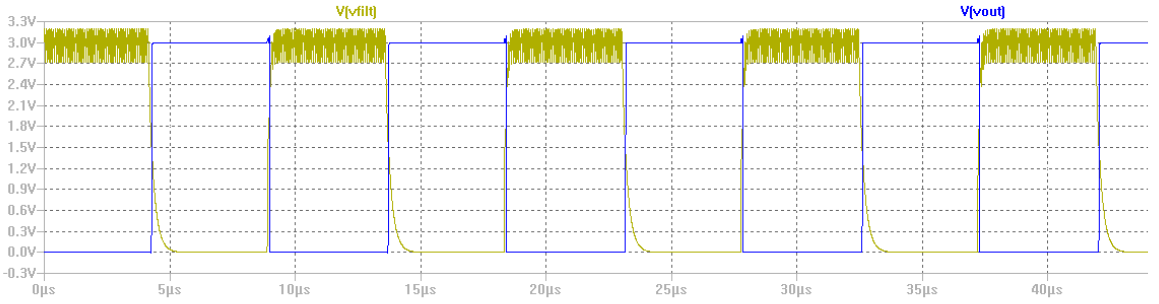
\includegraphics[scale=0.2]{Images/ImagenesTesina/Antecedentes/Sim_Schmit.png}
\caption{Input and output voltage of the Schmitt Trigger.}
\label{fig:Sim_Schmit}
\end{figure}

As a result of all the stages mentioned above, a Demodulator that operates according to fig. \ref{fig:Sim_demo} was obtained.

\begin{figure}[H]
\centering
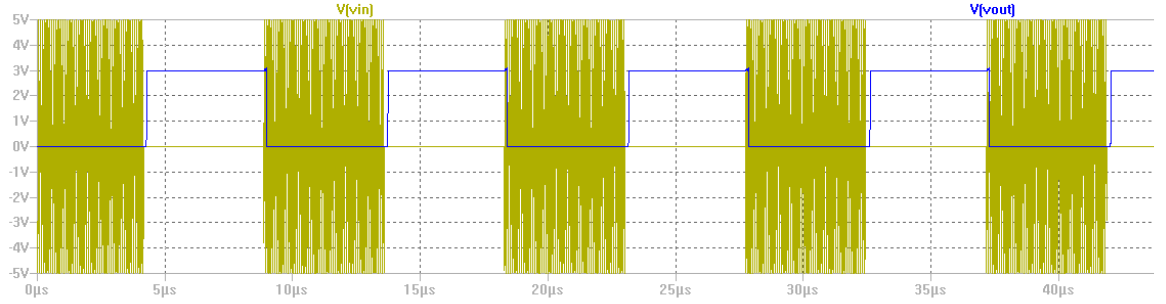
\includegraphics[scale=0.2]{Images/ImagenesTesina/Antecedentes/Sim_Demo.png}
\caption{Input and output voltage of the Demodulator.}
\label{fig:Sim_demo}
\end{figure}


\subsubsection{Final circuit}
Considering that, in practice, the high frequency noise present after the envelope detection stage did not complicate the subsequent logical tasks, the last stage (formerly formed by the Schmitt Trigger) only consisted of a buffer. See  \ref{fig:demod}.

\begin{figure}[H]
\centering
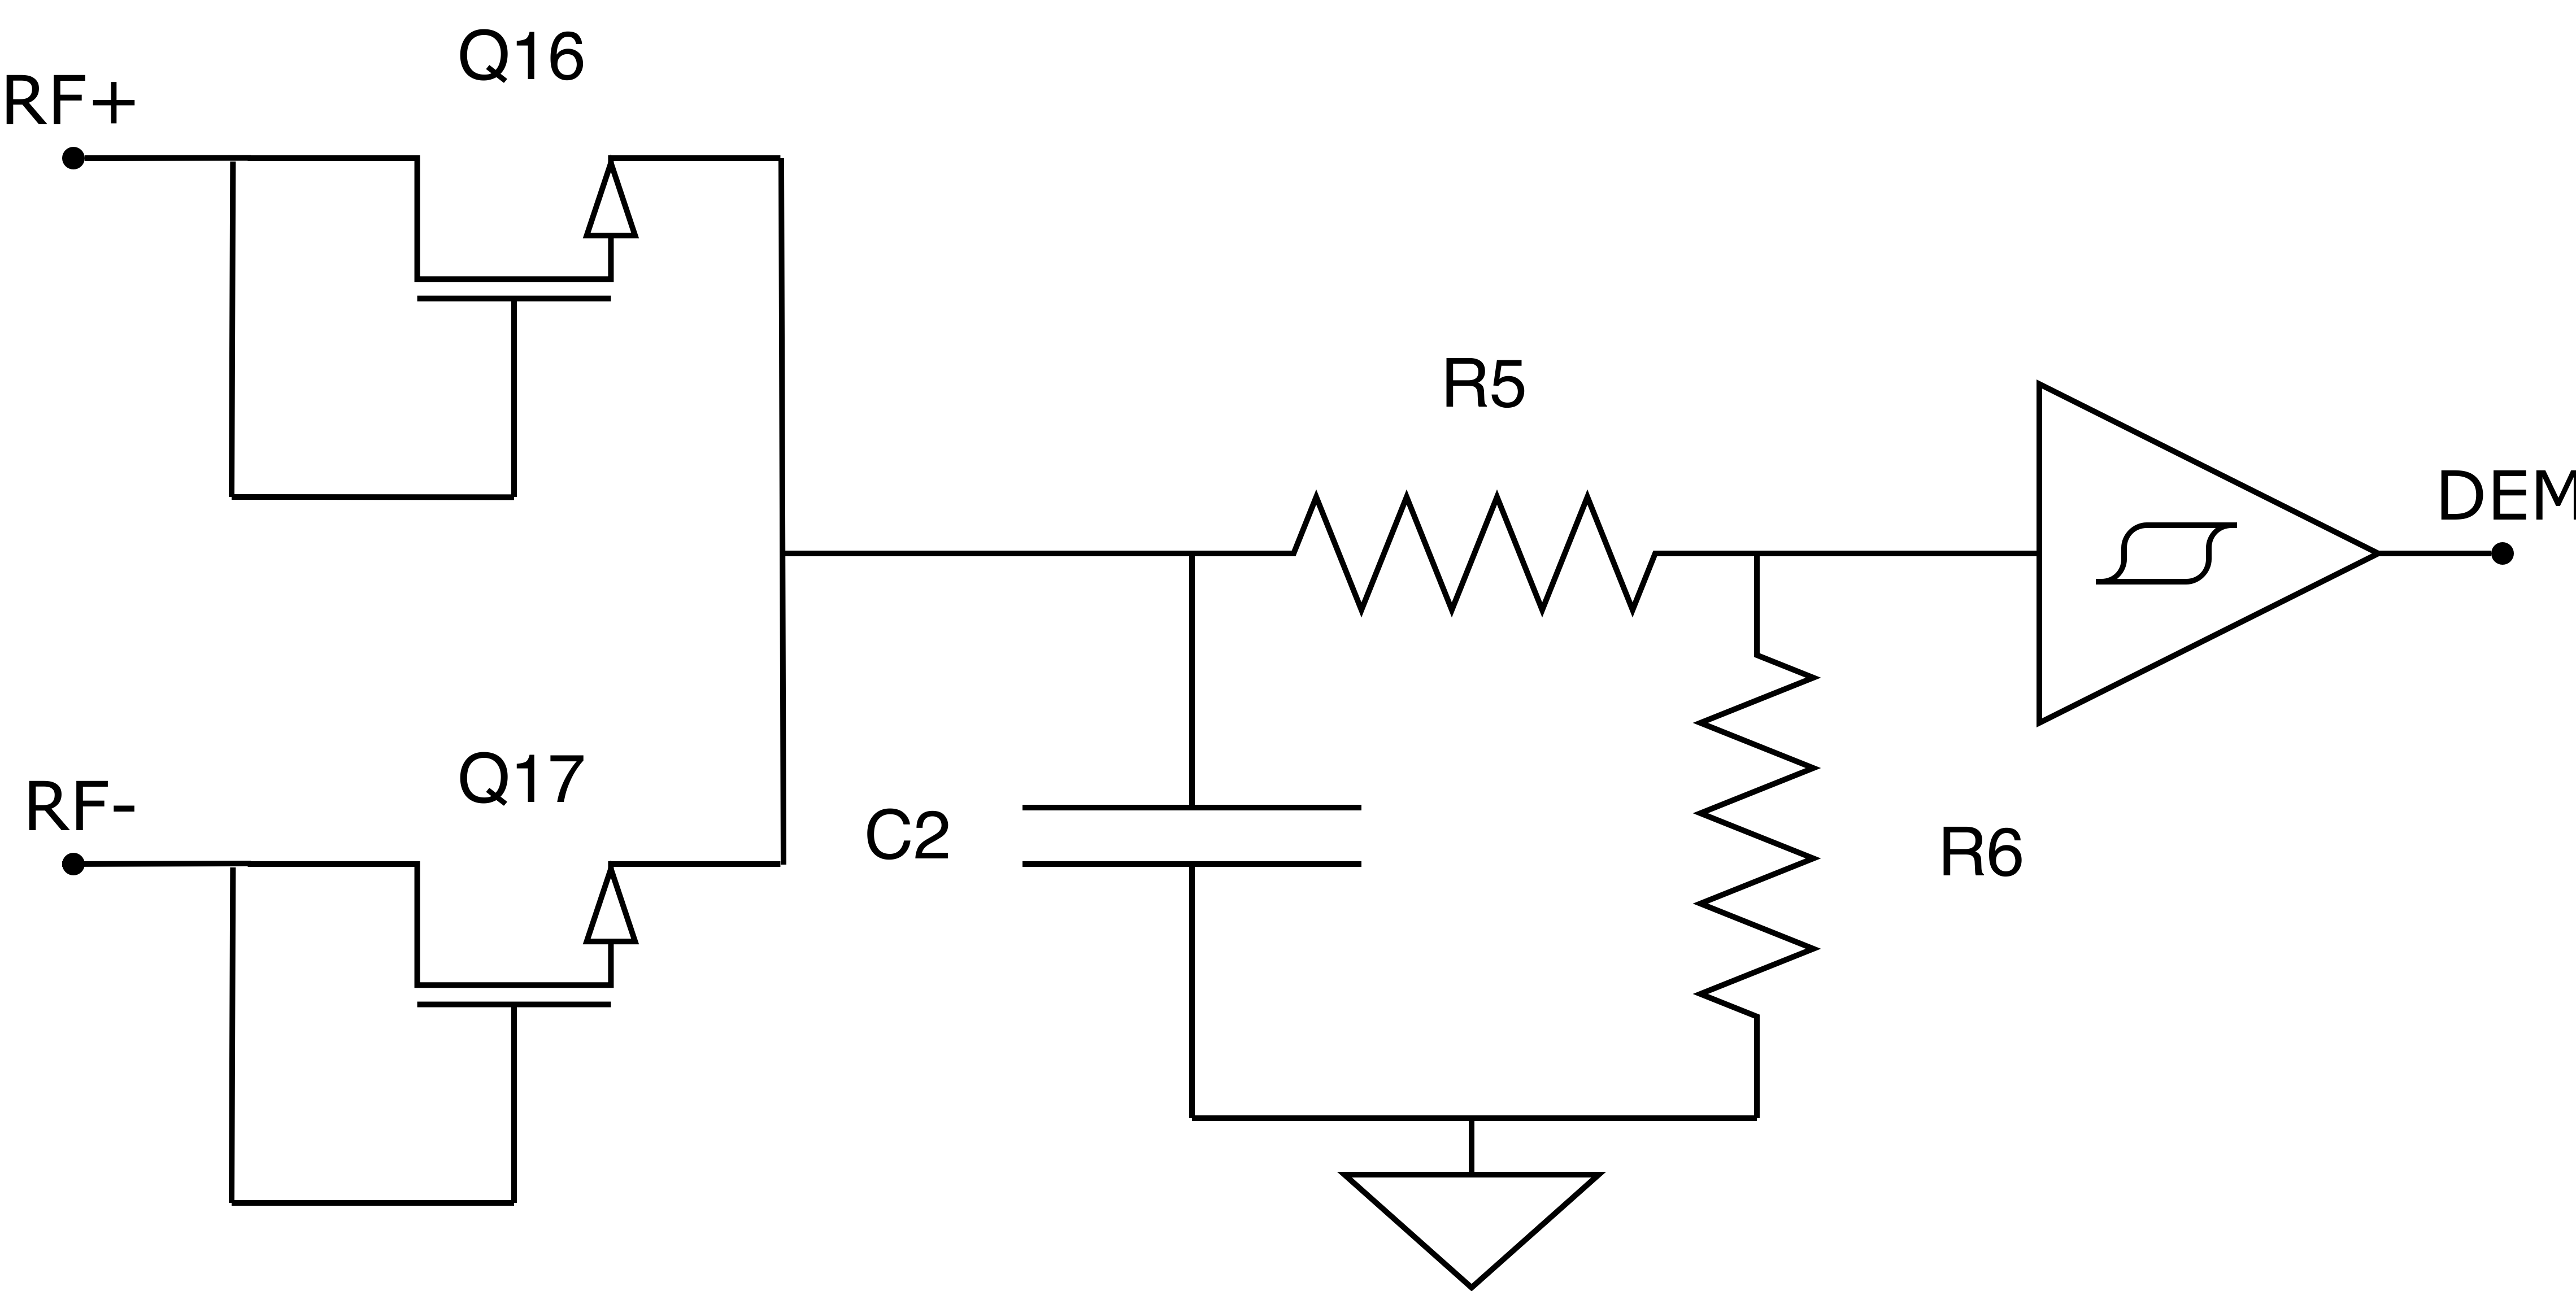
\includegraphics[width=0.7\linewidth]{Images/ImagenesTesina/circuitos/DEM.png}
\caption{Demodulator}
\label{fig:demod}
\end{figure}



\subsection{Power on reset (POR)}
This module is used to reset the digital machine (\textit{NFC Digital Core}) when the PICC approaches the PCD. The POR consists mainly of an RC low pass filter and a buffer. The schematic is shown in figure \ref{fig:por}.

\begin{figure}[H]


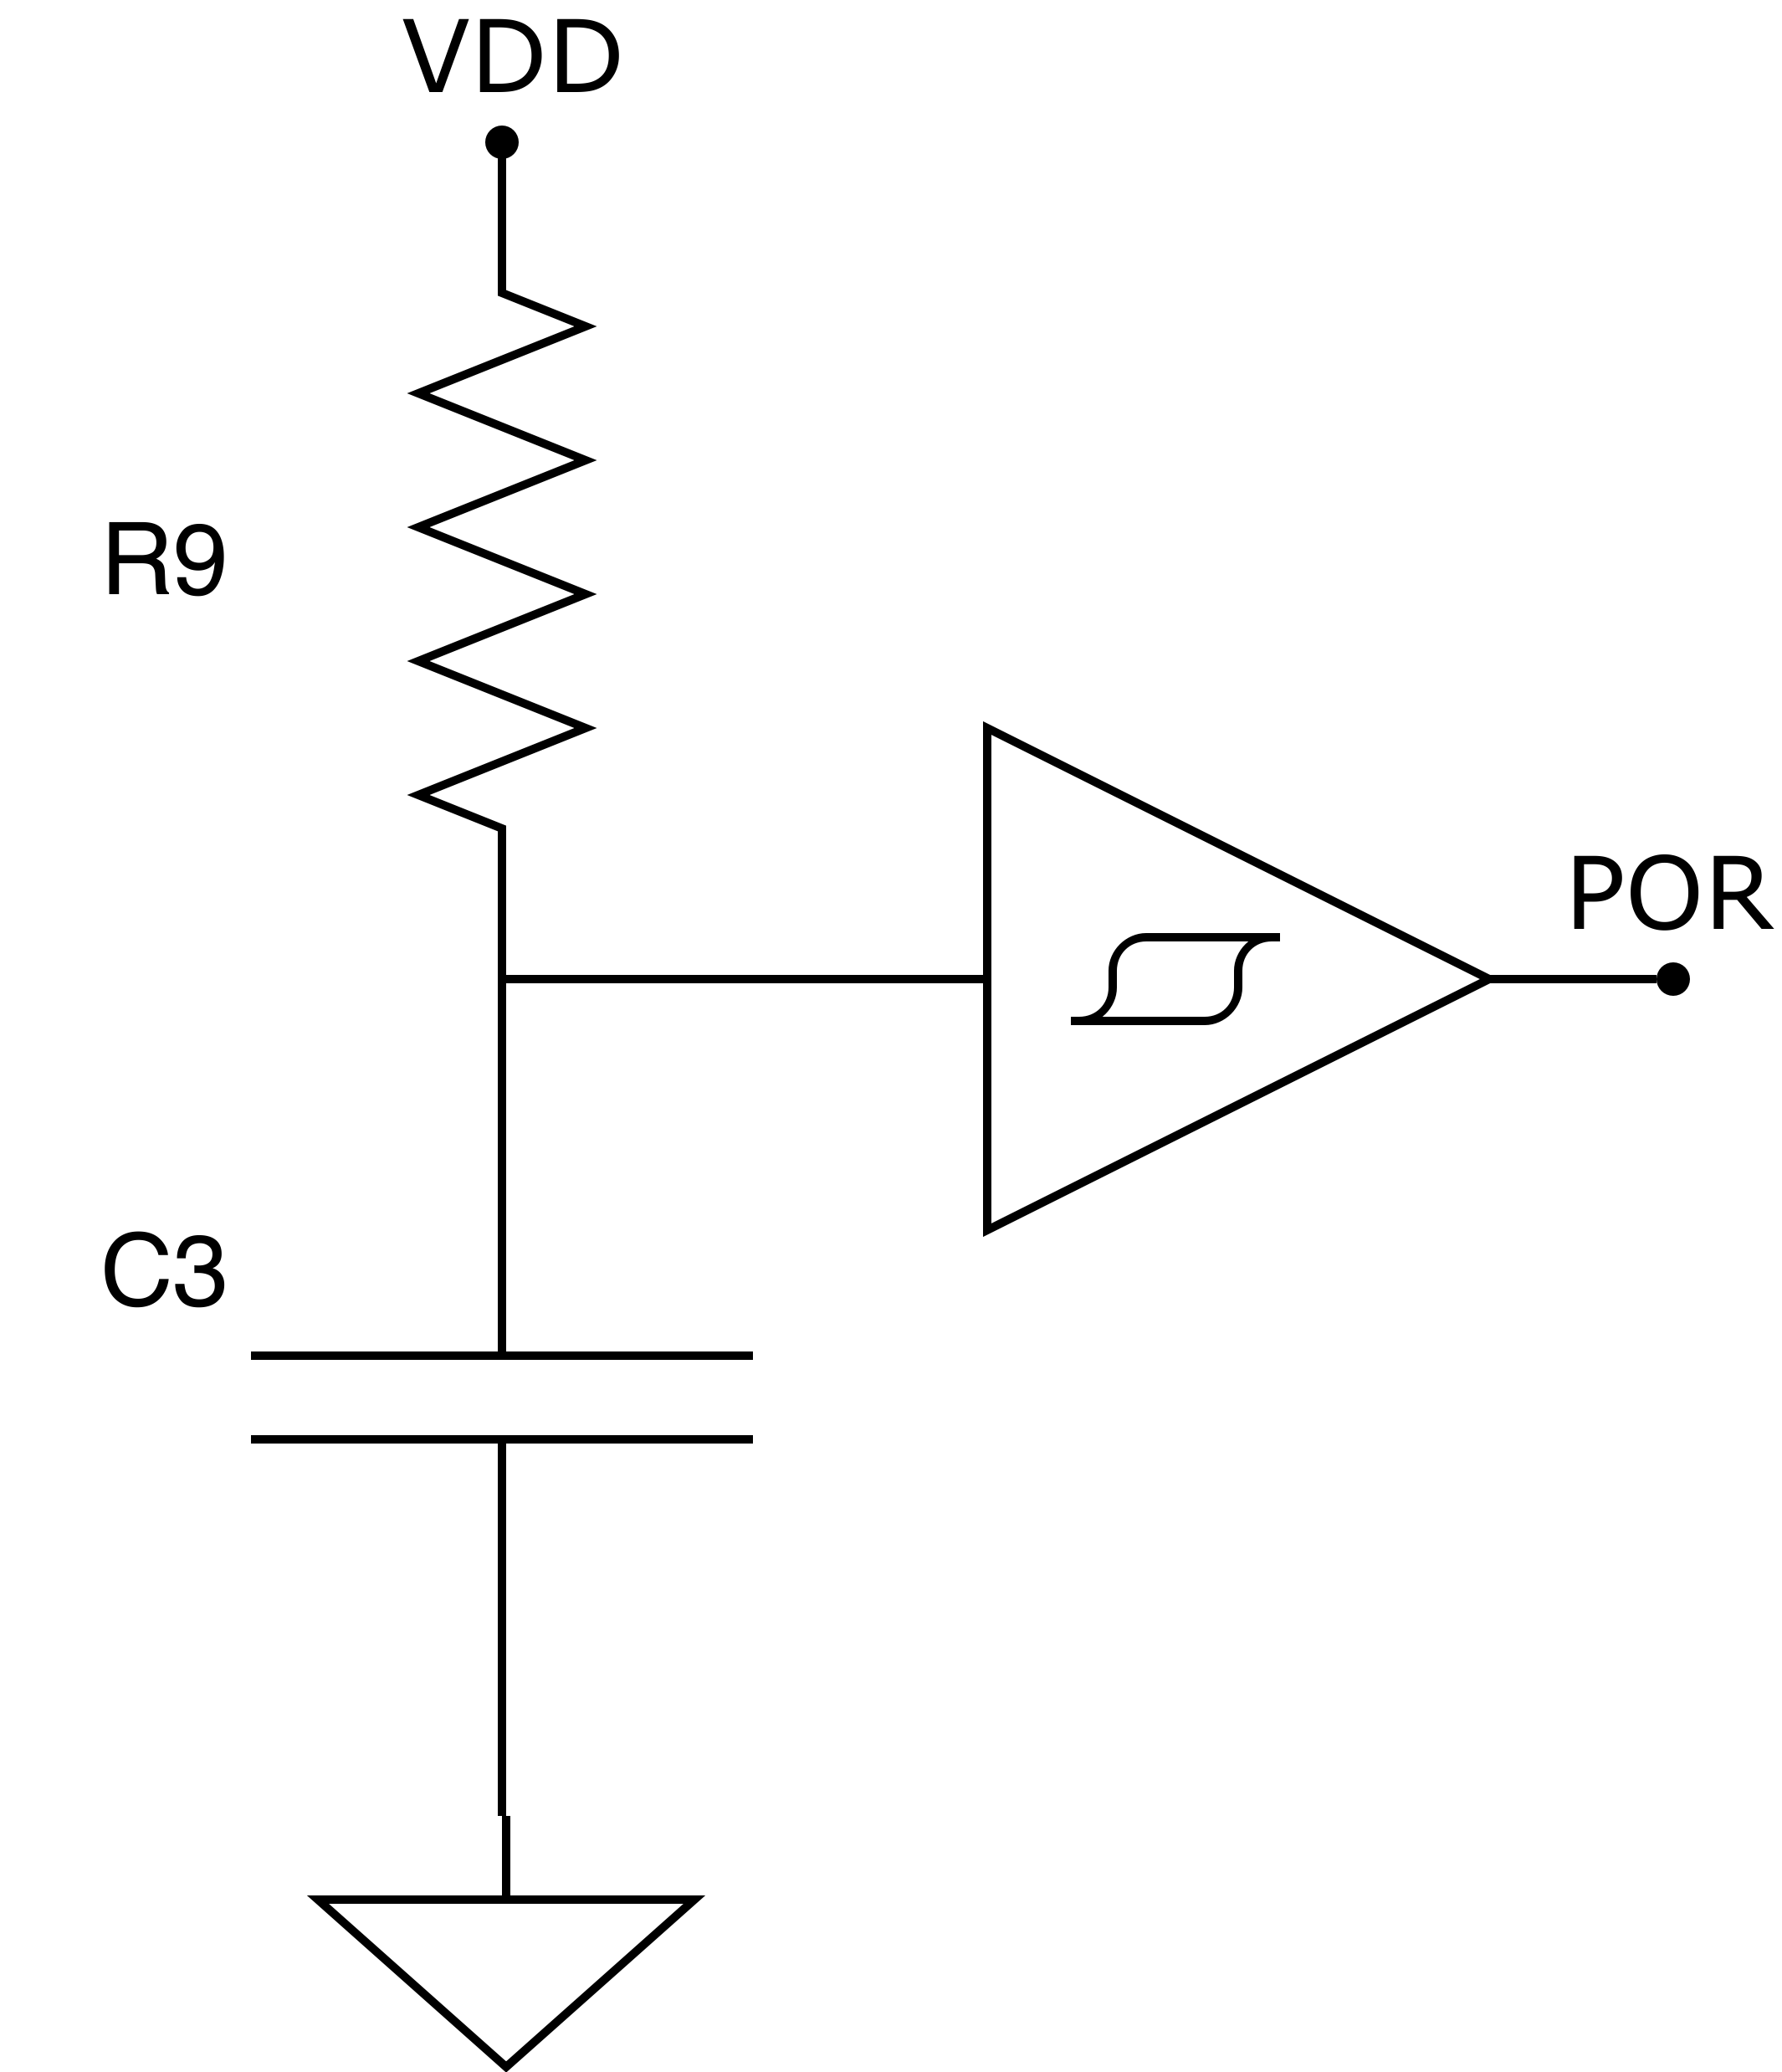
\includegraphics[width=0.3\linewidth]{Images/ImagenesTesina/circuitos/POR.png}
\centering
\caption{Power on reset}
\label{fig:por}
\end{figure}

\section{MEASUREMENT \& VALIDATION}
\subsection{Board for testing}
To carry out the measurements, a simple printed circuit was designed (Fig.   \ref{fig:500nm_test_placa}) to avoid dispersions by contact and by repeatability of measurements. It includes a DIP-40 socket for the integrated circuit and a low voltage drop regulator whose purpose is to power the IC ring pad. A 40 x 40 mm antenna of 4 turns was designed, with a 35 um copper thickness and set on an FR4 substrate, together with a trimmer to make fine-tuning adjustments.

\begin{figure}[H]
\centering
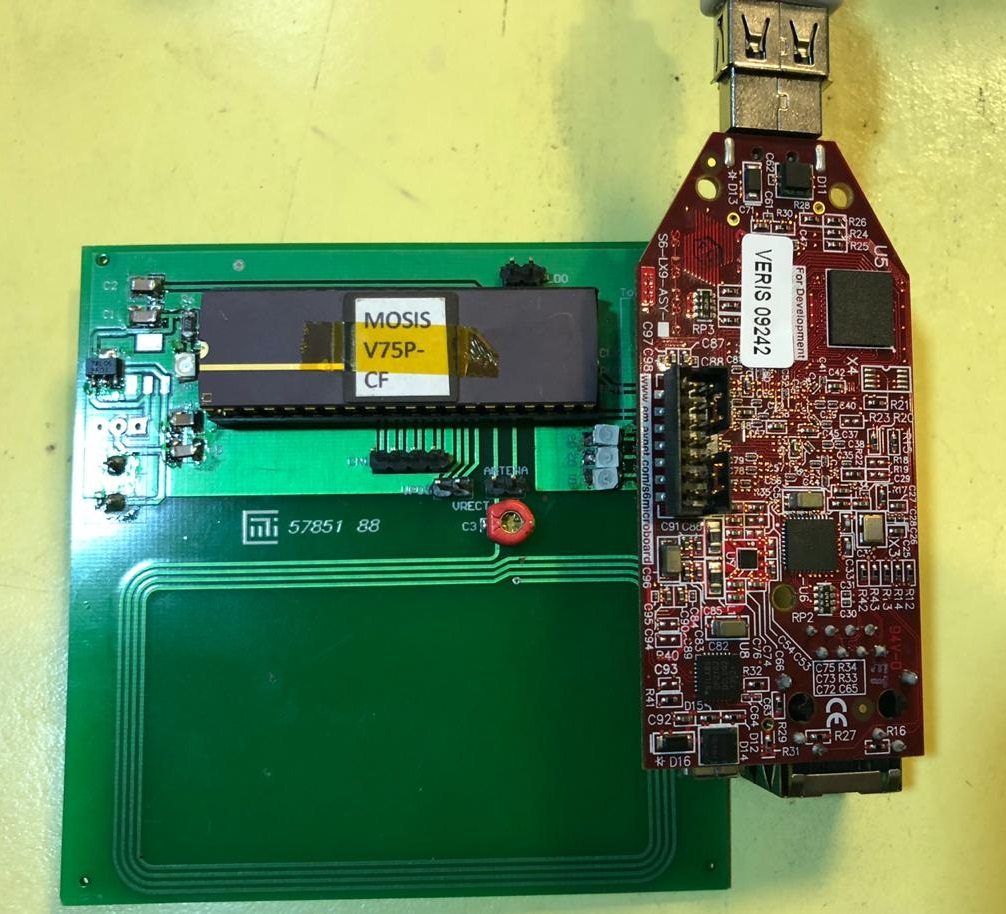
\includegraphics[scale=0.2]{Images/ImagenesTesina/500nm_Test_Shield.jpg}
\caption{Board for Front-End measurements.}
\label{fig:500nm_test_placa}
\end{figure}

\subsection{Antenna}
\subsubsection{Introduction}
This section contains the basic concepts of the antenna design for RFID applications. The following figure shows the RLC equivalent of an antenna:
% A lo largo de la guía se dan ejemplos para el cálculo de una antena con las siguientes
% características:
% \begin{itemize}
% \item Alambre de cobre de 0.3mm de diámetro.
% \item Número de espiras N = 5.
% \item 0,05 m de diámetro interior.
% \end{itemize}

% \begin{figure}[H]
% \centering
% 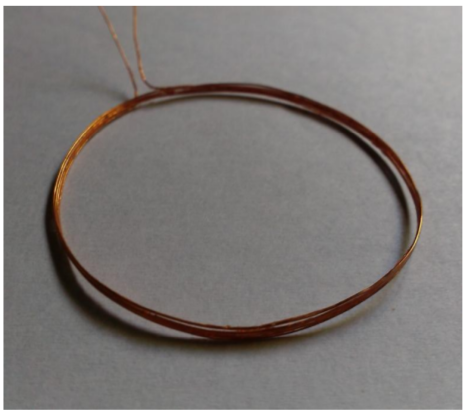
\includegraphics[scale=0.3]{Images/ImagenesTesina/antena/Antena.png}
% \caption{Antena diseñada.}
% \label{fig:antena}
% \end{figure}

\begin{figure}[H]
\centering
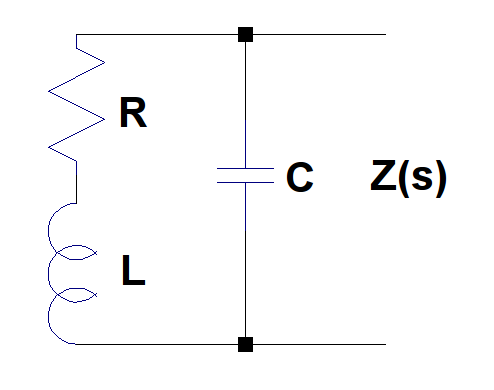
\includegraphics[scale=0.25]{Images/ImagenesTesina/antena/Antena_Equivalente.png}
\caption{PIC tuning circuit}
\label{fig:antena_eq}
\end{figure}

\subsubsection{Calculation of Resonance Frequency}



The circuit has an impedance of:

\begin{equation}
Z(S) = \frac{LS + R}{LCS^2 + RCS + 1}
\end{equation}

%
%De la cual luego de despejes matemáticos se obtiene la expresión de la frecuencia de resonancia:
%       No se si son necesarias las formulas
%
Sweeping along the  $j\omega$ axis $(S = j\omega)$ and multiplying by the conjugated number to separate the real part from the imaginary part: 

{\tiny{
$$ Z(S)|_{S=j\omega} = \frac{j\omega L + R}{-LC\omega ^2 + j\omega RC + 1}$$
$$Z(S)|_{S=j\omega} = \frac{R + j\omega L}{(1 - LC\omega^2) + j\omega RC} * \frac{(1 - LC\omega ^2) - j(\omega RC)}{(1 - LC\omega ^2) - j(\omega)}$$
$$Z(j\omega) = \Omega + jX = \frac{R(1 - LC\omega ^2)-jR^2C\omega+j\omega L(1-LC\omega ^2)+\omega ^2 RLC}{(1 - LC\omega ^2)^2 - (RC\omega )^2}$$
$$Z(j\omega) = \Omega + jX = \frac{R(1 - LC\omega ^2)+\omega ^2RLC}{(1 - LC\omega ^2)^2 - (RC\omega )^2}+j\frac{\omega L(1 - LC\omega ^2)-R^2C\omega}{(1 - LC\omega ^2)^2 - (RC\omega )^2}$$
.}}
The resonance frequency is reached when the imaginary part of the impedance becomes null, this is, $X(j\omega _o) = 0$

$$X(j\omega _o) = \omega _o L(1 - LC\omega _o ^2)-R^2C\omega _o = 0$$
$$X(j\omega _o) = L(1 - LC\omega _o ^2)-R^2C = 0$$

\begin{equation}
\omega _o = \sqrt[]{\frac{R ^2C - L}{L^2C}}
\end{equation}

For RFID antenna design, it is necessary to consider the Q of the inductor, since we are interested in how selective the antenna is. By definition $Q = \frac{\omega L}{R}$, where Q is the selectivity of the resonant circuit, $\omega$  the angular frequency, L the inductance and R the resistance (losses) of the antenna.

\begin{figure}[H]
\centering
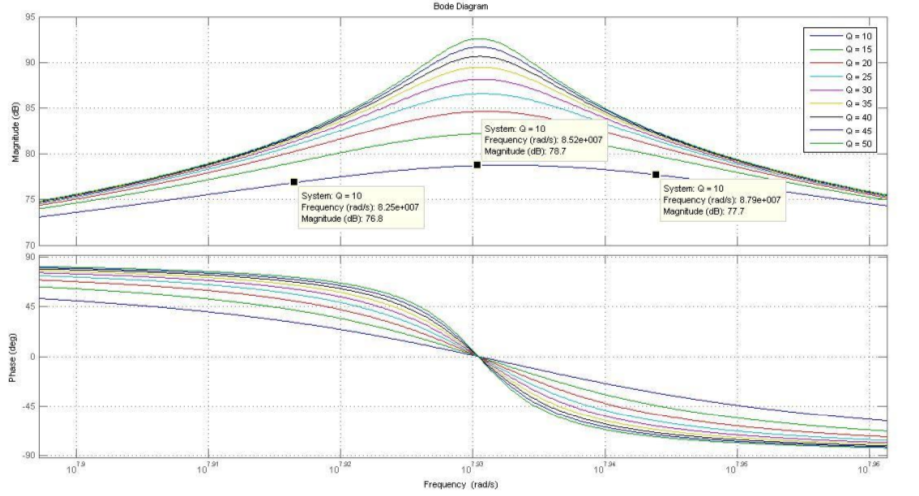
\includegraphics[scale=0.25]{Images/ImagenesTesina/antena/Respuesta_Frecuencia.png}
\caption{Frequency response of the tuning circuit.}
\label{fig:transf_frec}
\end{figure}

For communication from the PICC to the PCD, the carrier is modulated with ASK (Amplitude Shift Keying) at a frequency of 847 kHz. This creates two lateral bands in the spectrum around the central frequency. Figure \ref{fig:transf_frec} shows that with a Q of 10, the response drops approximately 1 dB. If Q is increased the circuit becomes more selective, filtering the sidebands and thus losing the modulation. According to  \cite{c8}, the quality factor must be:
\begin{equation}
{Q \leq \frac{f_c}{2B}}
\end{equation}
Being $f_c$ the central frequency (in this case 13.56MHz) and B the bandwidth. The optimal Q for ISO 15693 is $9\leq Q\leq 16$.
Therefore, for this design, a Q of 10 is chosen.

\subsubsection{Induced tension in the coil}
Based on magnetism laws, the induced voltage in the inductor is:
\begin{equation}
V = -N\frac{d\phi}{dt}
\end{equation}
\begin{equation}
\phi = \int_{}^{}  B \, dS
\end{equation}
Assuming that B, S and $\psi$ are constants in the interval analyzed, we get the following formula:

\begin{equation}
{V = 2 \pi fNBS\cos(\alpha)}
\end{equation}
Where f is the working frequency, N the number of turns, B the magnetic flux density, S the area of the coil and $\alpha$ the angle between the PICC and the PCD.

% \underline {Ejemplo:} \newline
% $$f = 13.56 MHz ; \alpha = \frac{\pi}{2}$$
% $$S = \pi (0.025m^2) = 1.96*10^{-3}$$
% $$1.5 < H < 7 [\frac{A}{m}]$$
% Entonces:
% $$0.315*N < V < 1.469*N  [Volts]$$
% Puede observarse que la tensión inducida en la bobina es directamente proporcional al número de espiras. Si N = 5, la tensión inducida estará comprendida, aproximadamente, entre 1.575 y 7.345 Volts.

\subsubsection{DC resistance of the antenna}
The resistance depends on the material and its geometry. It is directly proportional to the length and inversely proportional to the area:
\begin{equation}
{R_{DC} = \rho \frac{l}{S}}
\end{equation}
\newline
Being $\rho$  the resistivity of the material, l the length and S the area.

% \underline {Ejemplo:}\newline

% Se desea calcular la resistencia en continua de una bobina de cobre. La bobina tiene un
% diámetro de 0,05m, y la sección del cable es 0,3mm.

% $$ R_{DC} = \rho _{cu}\frac{l}{S} $$
% $$ R_{DC} = \frac{0.017 \Omega mm^2}{m}\frac{N 0.05m \pi}{\pi (0.15mm)^2} $$
% $$ R_{DC} = 0.03 \wideparen{7} N \Omega $$
% Para un N igual a 5:
% $$ R_{DC} = 0.1 \wideparen{8} \Omega $$

\subsubsection{AC resistance of the coil}
AC resistance of the coil. At high frequencies, the current density is larger near the surface of the conductor and decreases with greater depths in the conductor. This effect is called skin depth $\delta$.
According to  \cite{c9}, if the radius of the conductor and the depth of penetration are known, resistance can be approximated. The depth of penetration is:

\begin{equation}
{\delta = \frac{1}{\sqrt[]{\pi f \mu \sigma }}}
\end{equation}

Where f is the frequency, $\mu$ the permeability of the material and $\sigma$ the conductivity. For a copper wire at a working frequency of 13.56MHz, the depth of penetration is 0.018 mm. The resistance in AC is, then:

\begin{equation}
{R_{ac} = R_{DC} \frac{a}{1\delta}}
\end{equation}
$R_{DC}$ is the DC resistance, and 'a' the radius of the conductor.

% Siguiendo el ejemplo anterior, se tiene:

% $$ R_{ac} = 0.18 \frac{0.15}{2*0.018} \Omega = 0.75 \Omega $$

\subsubsection{Inductance of a coil of N turns}

\begin{figure}[H]
\centering
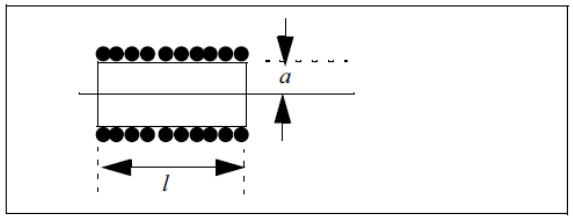
\includegraphics[scale=0.3]{Images/ImagenesTesina/antena/Bobina_N_Espiras.png}
\caption{Geometry of an N-turn coil}
\label{fig:N_esp}
\end{figure}

The inductance of a coil depends mainly on its geometry and the number of turns. 
According to \cite{c9}, the inductance L can be computed as:

\begin{equation}
{L = \frac{(aN)^2}{22.9 a+25.4 l}}
\end{equation}
\newline
Where a is the radius of the coil, l is the length, and N is the number of turns.
%\underline {Ejemplo:}\newline

%Se desea calcular la inductancia de una bobina con las siguientes especificaciones.

%\begin{itemize}
%\item a = 25mm
%\item l = 0.3mm N
%\item N = 5
%\end{itemize}

%$$ L = \frac{(25mm*5)^2}{22.9*25mm+25.4*0.3mm*5}\mu Hy = 25.59 \mu Hy $$

\subsubsection{Calculation of the quality factor or selectivity Q}
The quality factor is computed as:

\begin{equation}
{Q =\frac{\omega L}{R_{ac}}}
\end{equation}
%\underline{Ejemplo:}\newline
%Para los valores de L y R calculados anteriormente, hallar Q.
%\begin{itemize}
%\item $L = 25.59 \mu Hy$
%\item $R_{ac} = 0.75 \Omega$
%\item $\omega = 2\pi *13.56MHz$
%\end{itemize}

%$$ Q = \frac{2\pi *13.56MHz*25.59\mu Hy}{0.75 \Omega} = 1907 $$

%\subsubsection{Mediciones del solenoide de 5 espiras}
\subsubsection{Prototype antenna measurements}
Prior to the printed circuit production, which was mentioned in the previous subsection, an antenna was built, as seen in fig \ref{fig:L_real}. Specifically a 5-turn solenoid was made and it was measured with a RLC meter (Tonghui TH2826A). Then the values obtained were contrasted with an analogous Q meter.

\begin{figure}[H]
\centering
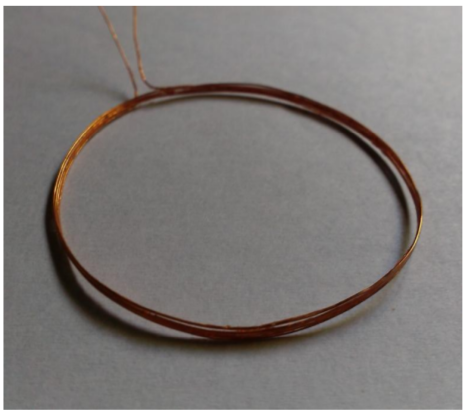
\includegraphics[scale=0.3]{Images/ImagenesTesina/antena/Antena.png}
\caption{Designed antenna.}
\label{fig:antena}
\end{figure}
% Se fabricó una antena con las características mencionadas al principio de la guía, y se midió
% con un medidor RLC (Tonghui TH2826A). Luego se contrastaron los valores con un Qmetro
% analógico.

\begin{figure}[H]
\centering
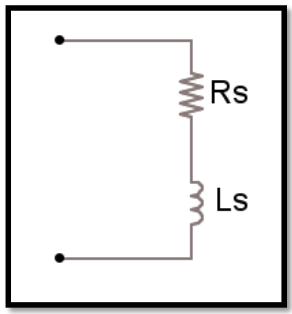
\includegraphics[scale=0.4]{Images/ImagenesTesina/antena/Equivalente_Bobina_Serie.png}
\caption{Equivalent circuit of the real inductor.}
\label{fig:L_real}
\end{figure}


The following data were obtained:

\begin{table}[H]
\centering
\caption{MEASUREMENTS OF THE ANTENNA}
\label{table:med_antena}
\begin{tabular}{c|c|c|c}
\textbf{Frequency  [Hz]} & \textbf{Ls [Hy]}       & \textbf{Rs [$\Omega$]} & \textbf{Q}                                                                                \\ \hline
1000                    & 2.9039E-06 & 0.2648   & 0.06890291                                                                             \\
2000                 & 3.3124E-06 & 0.278   & 0.14972785                                                                             \\
100000                  & 3.2564E-06 & 0.2776   & 7.37061094                                                                                 \\
200000                  & 3.2404E-06 & 0.3012   & 13.5193621                                                                             \\
500000                  & 3.2262E-06 & 0.374   & 27.0998486                                                                             \\
800000                  & 3.1978E-06 & 0.4432   & 36.2680427                                                                             \\
1000000                  & 3.1899E-06 & 0.4705   & 42.598928                                                                             \\
200000                  & 3.0715E-06 & 0.7688   & 50.2041871          
\end{tabular}
\end{table}

\begin{figure}[H]
\centering
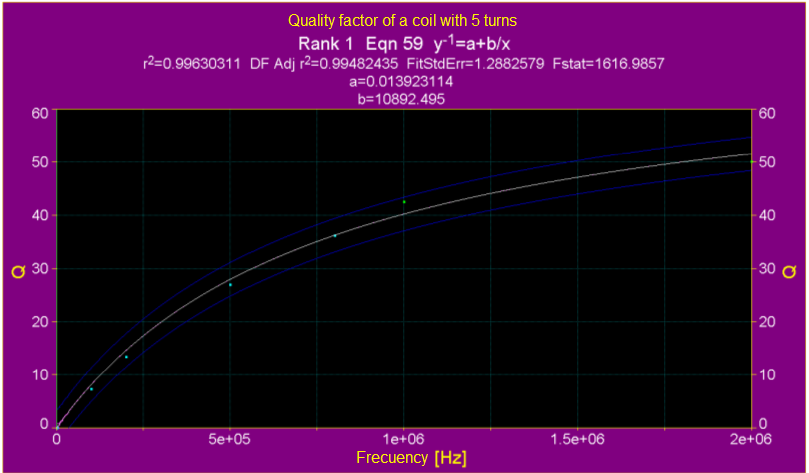
\includegraphics[scale=0.4]{Images/ImagenesTesina/antena/Simulacion_Q_Antena_2.png}
\caption{Variation of the coil's Q in relation to the frequency.}
\label{fig:L_Qsim}
\end{figure}

Adjusting the curve, Q varies approximately in the following way:

\begin{equation} \label{eq:vref}
 Q = \frac{1}{a + \frac{b}{f}} = \frac{1}{0.0139 + \frac{10892.495}{f}} 
\end{equation}


At the frequency of interest (f = 13.56 MHz):
$$Q = 67.90528 \pm 3.152254 \textrm{; 95\% confidence interval } $$ 

\subsubsection{ Antenna for testing}
In order to carry out the integrated circuit laboratory tests an antenna was built based on ISO/IEC10373 \cite{c7} standards  (fig. \ref{fig:L_test}).
The inductance shown by this antenna was $1.6 \mu Hy$, and a necessary parallel capacity of $88 pF$ for a resonance frequency of 
$13.56 MHz$.


\begin{figure}[H]
\centering
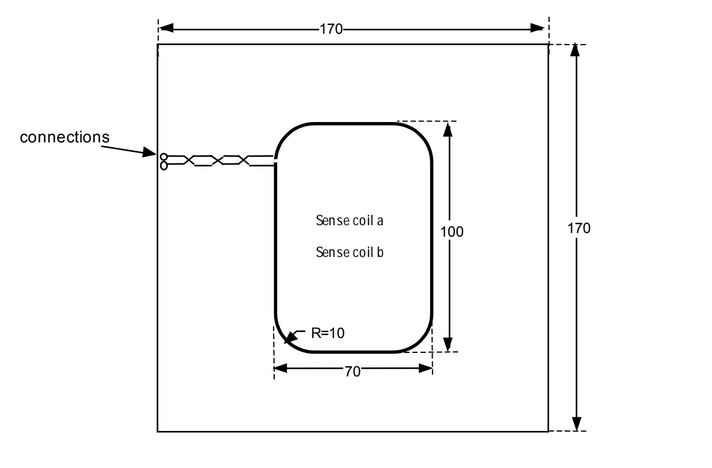
\includegraphics[scale=0.45]{Images/ImagenesTesina/antena/Bobina_Testing.JPG}
\caption{Antenna for testing (ISO / IEC10373).}
\label{fig:L_test}
\end{figure}




\subsection{Analog Front-End measurements}
In order to verify and validate the design, each module
is tested and compared with simulation results. The
corresponding tests verify the feasibility of the design.
The measurement of the clock generator and a phase of
the RF field (RF+) is shown in the Fig. \ref{fig:clock_medicion}. 

\begin{figure}[H]
    \centering
    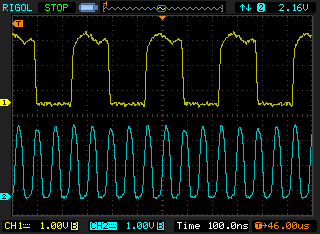
\includegraphics[scale=0.5]{Images/ImagenesTesina/mediciones/clk.png}
    \caption{Clk/4 vs RF+}
    \label{fig:clock_medicion}
\end{figure}

The wave demonstrates that the CG works well and can divide the clock 13.56MHz/4. The ripple of the clock is due to the noise of
external power source which the ring pad is connected to
Fig. \ref{fig:por_medicion} shows the comparison between RF+ with the output of the POR module. It can be seen the delay of the
POR in relation to the input signal. This delay allows the
DPU changing to the idle state.

\begin{figure}[H]
    \centering
    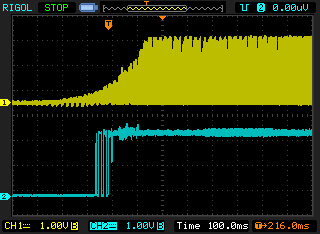
\includegraphics[scale=0.5]{Images/ImagenesTesina/mediciones/por.png}
    \caption{RF+ vs POR}
    \label{fig:por_medicion}
\end{figure}


Finally, Fig. \ref{fig:demod_medicion} shows the signal recovery transmitted from
PCD. It demonstrates that the clock is interrupted when a
frame arrives.

\begin{figure}[H]
    \centering
    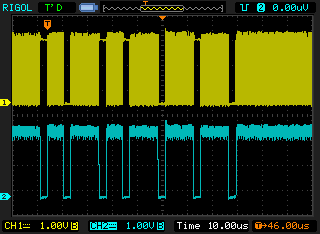
\includegraphics[scale=0.65]{Images/ImagenesTesina/mediciones/demod2.png}
    \caption{Clk/4 vs Demodulator}
    \label{fig:demod_medicion}
\end{figure}


\section{IC CIRCUIT FLOORPLANING}

The corresponding layout is shown in Fig. \ref{fig:chip GF130} and Fig. \ref{fig:layout GF130}
designed for Global Foundries 130nm CMOS process. The
analog Front-End covers 0.3mm x 0.2mm (Fig. \ref{fig:layout GF130}).
The GF130 design, explained in this paper, was
manufactured by MOSIS \cite{mosis} and it is shown in Fig. \ref{fig:chip GF130}. The
next section will explain the conclusions made about the measurements and tests performed on this integrated circuit.


\begin{figure}[H]
    \centering
    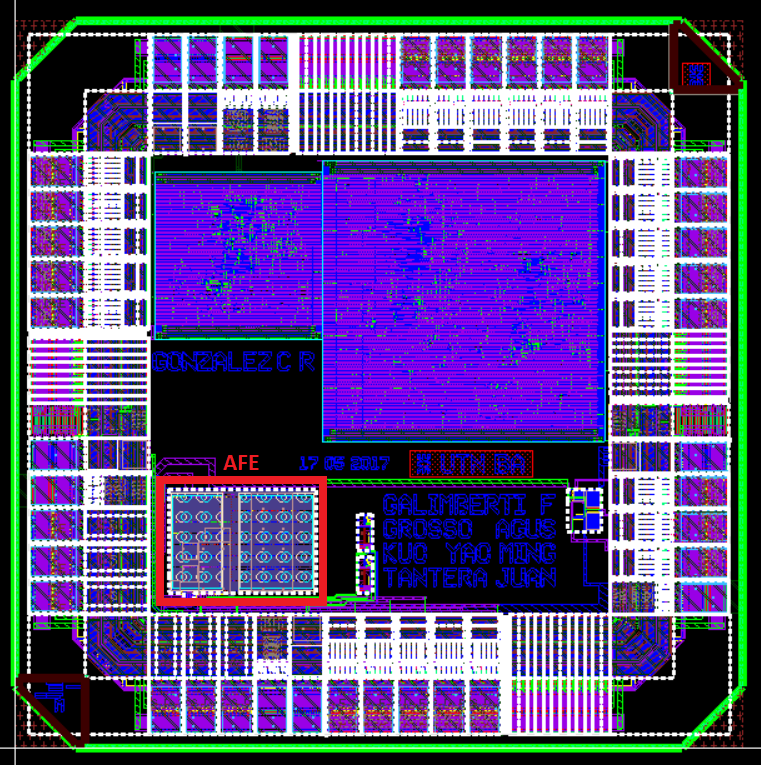
\includegraphics[width=0.5\linewidth]{Images/ImagenesTesina/circuitos/gf130_layout.png}
    \caption{GF130 Layout}
    \label{fig:layout GF130}
\end{figure}

\begin{figure}[H]
    \centering
    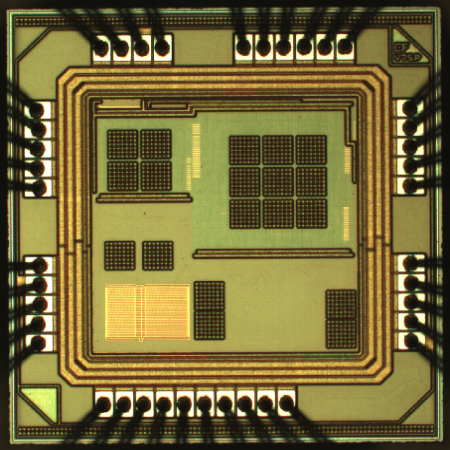
\includegraphics[width=0.5\linewidth]{Images/ImagenesTesina/chip_130.png}
    \caption{GF130 Chip}
    \label{fig:chip GF130}
\end{figure}


\section{Conclusion}
An Analog Front-End circuit for ISO/IEC14443A compatible
RFID transponder IC was designed and implemented by using
the Global Foundries 130nm (eight-metal/mim-capacitor)
CMOS process. Measurements demonstrated that the
transponder IC works properly (converts RF power to DC
voltage, extracts the clock and data, and  sends data back correctly). Using GF130 could drastically reduce the area
in comparison with older technologies. This is a huge
improvement compared with the existing products.

\paragraph{Conflict of Interest}

The authors declare no conflict of interest.

\section{Acknowledgment}
The authors would like to thank to Nanolab - UTN FRBA for their support and to the Centro de Micro y Nano Electronica del Bicentenario (CMNB-INTI) \cite{inti} for their contributions and the use of the testing facilities. We also thank MOSIS and Synopsys academic programs. The integrated circuit was designed using Synopsys \cite{synopsys} tools under the Synopsys University Program. The chips were fabricated through the MOSIS foundry service supported by the MOSIS Educational Program (MEP).


\paragraph{References}

\newline

\footnotesize{

 
%\begin{enumerate}
\begin{thebibliography}{99}
\bibitem{journal1}
	M. Uzunoglu, M. S. Alam, ``Dynamic modeling, design, and simulation of a combined PEM fuel cell and ultracapacitor system for stand-alone residential applications" IEEE Trans. Ener. Conv., \textbf{21}(3), 767--775, 2006. https://doi.org/10.1109/TEC.2006.875468


\hspace{-1cm} \textbf{Conference Papers:}

\bibitem{c3}
	Valentin Chesaru and Antonio Pieleanu and Claudius Dan and Mircea Bodea, RFID 13.56MHz TRANSPONDER IC FRONTEND, 2010.

\bibitem{c4}
	Jie Tian and Zhongchen Yu, Analog Front End Design of Contactless Smart Card, 2012.

\bibitem{c5}
	Sebastián Pazos, Fernando Aguirre, Tomás Mazur, G. Peretti and E. Romero, Evaluación de la calidad de TRAM en la detección de fallas de fabricación en circuitos integrados analógicos fabricados en tecnología CMOS de 500nm, Universidad Tecnológica Nacional, Facultad Regional Buenos Aires y Universidad Tecnológica Nacional, Facultad Regional Villa María. 2015.

\bibitem{c6}
	Munish Kumar, Parminder Kaur, Sheenu Thapar, Design of CMOS Schmitt Trigger, International Journal of Engineering and Innovative Technology (IJEIT). 2012.

\bibitem{c10}
	Chao Lu and Yong-ming Li, The RF Interface Circuits Design of Contactless IC Cards, 2001.

\hspace{-1cm} \textbf{Books:}

\bibitem{c1} 
	Klaus Finkenzeller, RFID Handbook - Fundamentals and Applications in Contactless Smart Cards and Identification 3rd Edition, 2010.

\hspace{-1cm} \textbf{Additional bibliography:}

\bibitem{c2}  
	Identification cards - Contactless integrated circuit(s) cards - Proximity cards, ISO/IEC Std. 14443.

\bibitem{c7}
	Identification cards - Test methods - Proximity cards, ISO/IEC 10373

\bibitem{c8}
	13.56 MHz RFID systems and antennas design guide, MELEXIS Microelectronic Integrated Systems, 2004.

\bibitem{c9}
	Dr. Youbok Lee, Ph.D., AN710 Antenna Circuit Design for RFID Applications, Microchip. 2003.

\bibitem{mosis}
	MOSIS Services, https://www.mosis.com/

\bibitem{inti}
	CMNB - INTI, http://www.inti.gob.ar/microynanoelectronica/cmnb.htm

\bibitem{synopsys}
	Synopsys, https://www.synopsys.com/

%\end{enumerate}
\end{thebibliography}{90}
\noindent

} 

\end{multicols}

\end{document}

